\section{ERP-ONE}

\subsection{About ERP-ONE}

ERP-ONE is a combined ERP/WMS software solution. ERP stands for Enterprise Resource Planning, and WMS stands for Warehouse Management System.

All day-to-day operations in the office and warehouse involve, in some part, the ERP-ONE software.

\subsection{Item Maintenance}

\subsubsection{Item Master Maintenance}

\index{ERP-One Commands!ITEM}

The \texttt{ITEM} command is used to access Item Master Maintenance.

\begin{enumerate}
	\begin{figure}[H]
		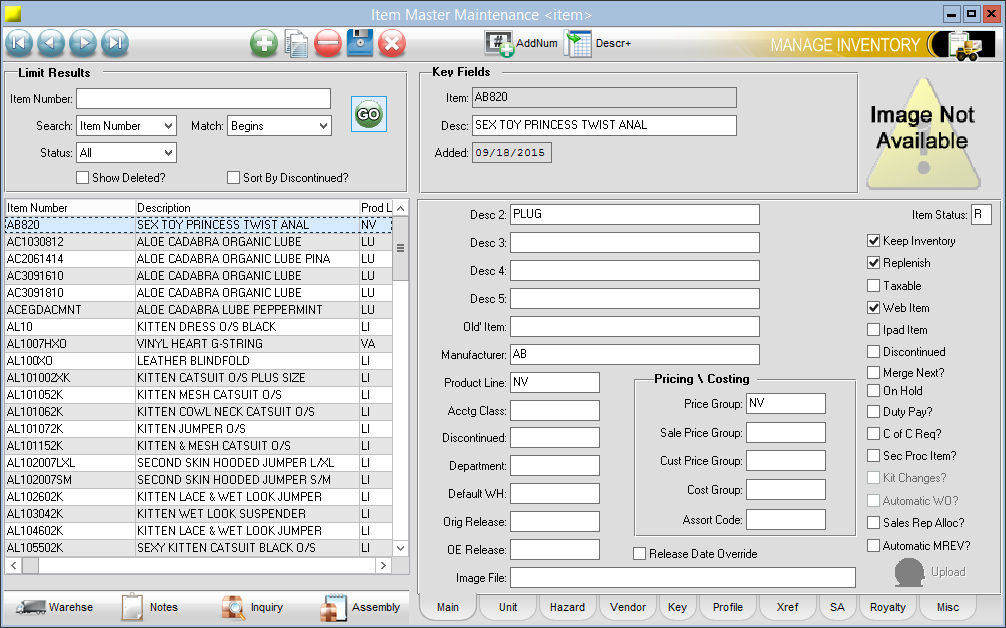
\includegraphics[width=\textwidth]{../img/image55}
		\caption{ITEM Item Master Maintenance Main Tab}
	\end{figure}
	\item Main Tab	
	\begin{itemize}
		\item Item \textemdash Enter item number of click on the add by number and it will give you the next available item number
		\item Desc. \textemdash Enter item description, 1-5 are available for item description, if there is data in the fields it will print on standard forms. Each description field is 30 characters long
		\item Old' Item \textemdash Cross reference field
		\item Product Line \textemdash Required field, pressing F1 in this field will open \texttt{ITPLM} double click on the product line and click enter
		\item Manufacturer \textemdash Open field to put in manufacturer's name or code
		\item Image File \textemdash Link image of product display in upper right hand corner and print on labels; imaghe file must be saved on server to activate and you may use the F1 browser to find the file
		\item Pricing \ Costing
		\begin{itemize}
			\item Pressing F1 in the following 4 fields opens \texttt{ITPG}
			\begin{itemize}
				\item Price Group \textemdash groups items together for pricing
				\item Sale Price Group \textemdash groups items for sale pricing
				\item Cust Price Group \textemdash groups items for special pricing
				\item Cost Group \textemdash groups items for purchase costing
			\end{itemize}
			\item Assort Code \textemdash Pressing F1 in this field opens \texttt{ITACDI} and allows you to set up items for quantity discount pricing
		\end{itemize}
		\item Item Status \textemdash Pressing F1 in this field opens System Help, so you can decide what item status you want. Enter the letter and click enter.
		\begin{itemize}
			\item R \textemdash Regular warehouse item
			\item S \textemdash Special item or for specific customers
			\item D \textemdash Obsolete "Discontinued" (also use checkbox \& date)
			\item A \textemdash Kit/assembly item
			\item N \textemdash Obsolete "Non Stock" or Drop Ship item
		\end{itemize}
		\item Checkboxes
		\begin{itemize}
			\item Keep Inventory \textemdash Keeps quantity count in \texttt{WAITM}
			\item Replenish \textemdash Will show on purchase order reports to buy
			\item Taxable \textemdash Items are usually taxable (Customer setup will determine final sales tax decision)
			\item Web item \textemdash Item is a web item for ecommerce
			\item Discontinued \textemdash Item is discontinued and auto populates current day into the discontinued date field when checked
			\item C of C Req. \textemdash Item includes a certificate of compliance			
		\end{itemize}		
	\end{itemize}
	\begin{figure}[H]
		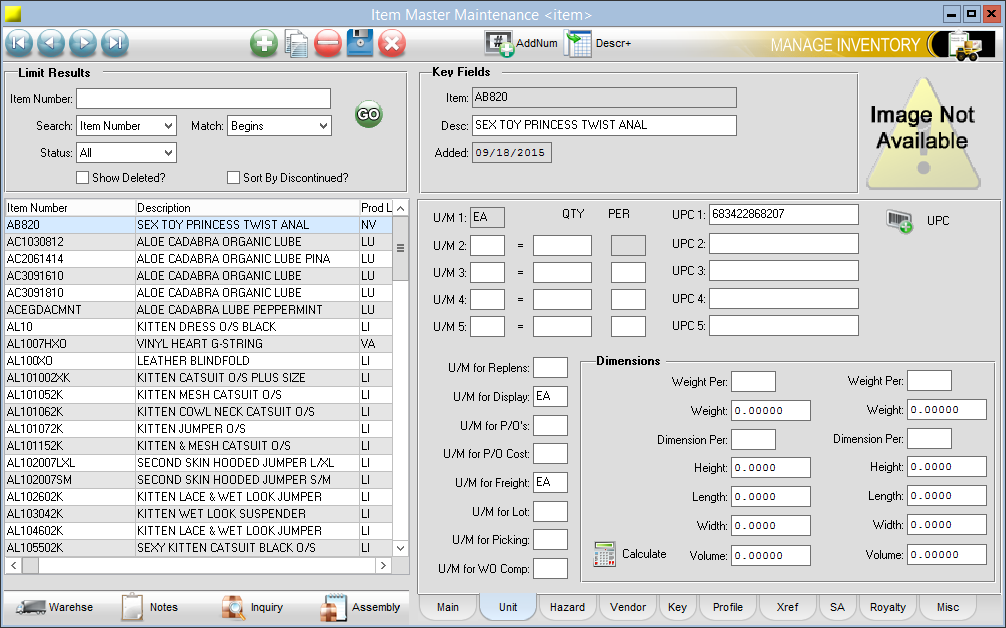
\includegraphics[width=\textwidth]{../img/image56}
		\caption{ITEM Item Master Maintenance Unit Tab}
	\end{figure}
	\item Unit Tab (requires \texttt{ITUMM} setup first)
	\begin{itemize}
		\item Unit of Measures required, start with smallest needed for item
		\begin{itemize}
			\item U/M 1 \textemdash A quantity used as a standard of measurement, starting with the lowest unit of measure \texttt{ITUMI}
			\item U/M 2-5 \textemdash Optional field, option U/M defaults
			\item QTY \textemdash The quantity of lower U/M for the U/M level chosen
			\item PER \textemdash Based on other U/M setup against item
			\item UPC \textemdash Universal Product Code for each U/M, optional
			\item U/M for Replens \textemdash U/M for replenishing inventory
			\item U/M for Display \textemdash U/M that displays in system, this will be the default for all if no other field is filled in
			\item U/M for P/O's \textemdash U/M for purchase orders
			\item U/M for P/O Cost \textemdash U/M for costing
			\item U/M for Freight \textemdash U/M for freight
			\item U/M for Lot \textemdash U/M for lots
			\item U/M for Picking \textemdash U/M for picking product
			\item U/M for WO Comp \textemdash U/M to use as Work Order Components
		\end{itemize}
		\item Dimensions / Weight Per \textemdash For shipping purposes
		\begin{itemize}
			\item Weight per \textemdash U/M
			\item Weight \textemdash Weight
		\end{itemize}
	\end{itemize}
	\begin{figure}[H]
		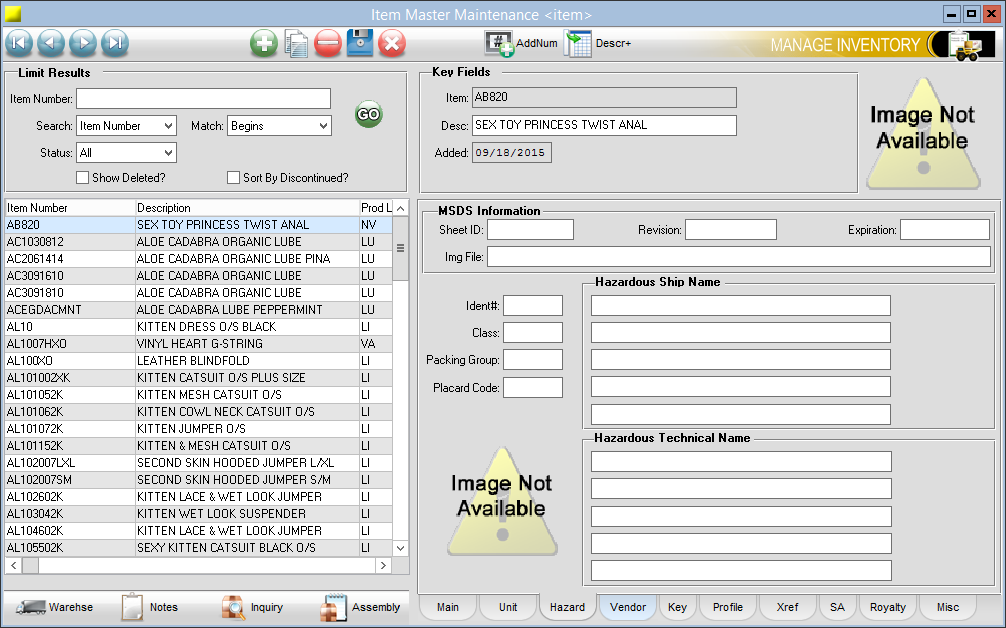
\includegraphics[width=\textwidth]{../img/image57}
		\caption{ITEM Item Master Maintenance Hazard Tab}
	\end{figure}
	\item Hazard Tab \\
	If item has hazardous material and requires an MSDS sheet, store data and link MSDS sheet. Image needs to be stored on server first.
	\begin{figure}[H]
		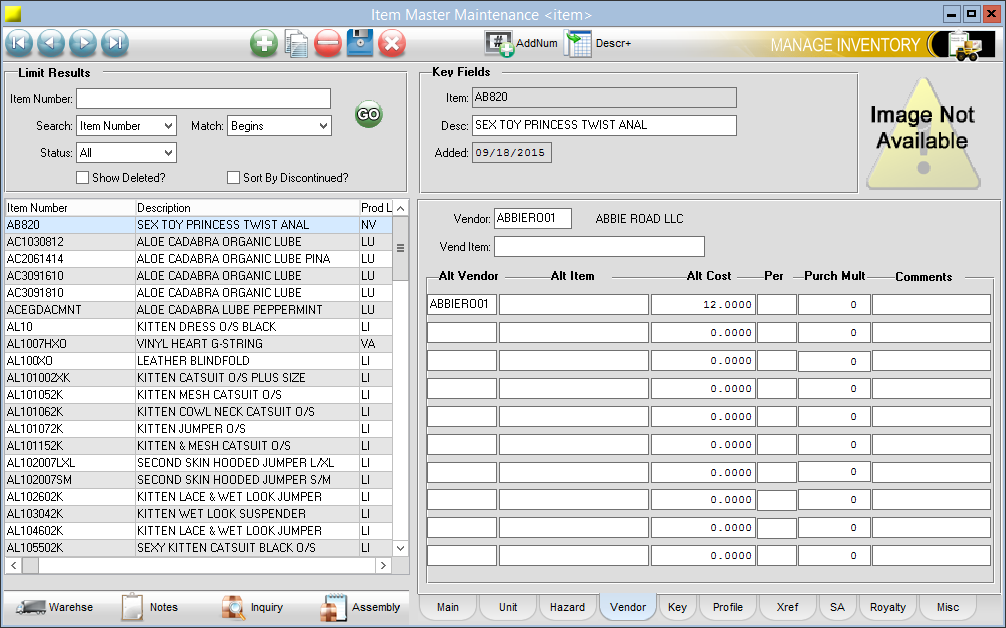
\includegraphics[width=\textwidth]{../img/image58}
		\caption{ITEM Item Master Maintenance Vendor Tab}
	\end{figure}
	\item Vendor Tab \textemdash To select primary vendor for this item
	\begin{itemize}
		\item Vendor \textemdash Enter primary vendor or use F1 to open \texttt{VEMM}
		\begin{itemize}
			\item Vend Item \textemdash Enter rpimary vendor part number, this is also a cross reference
		\end{itemize}
		\item Alt Vendor \textemdash Store alternative vendor for item, using F1 in this field opens \texttt{VEMM}
		\begin{itemize}
			\item Alt Item \textemdash Enter alternative item number
			\item Alt Cost \textemdash Enter alternative cost
			\item Purch Mult. \textemdash Quantity amount that vendor requires to purchase
		\end{itemize}
	\end{itemize}
	\begin{figure}[H]
		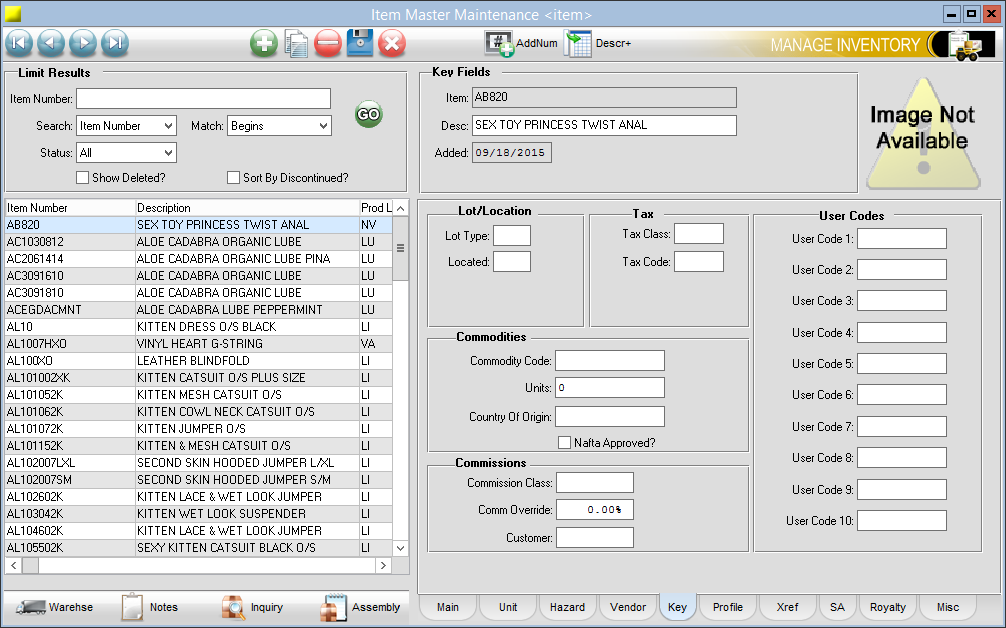
\includegraphics[width=\textwidth]{../img/image59}
		\caption{ITEM Item Master Maintenance Key Tab}
	\end{figure}
	\item Key Tab
	\begin{itemize}
		\item Lot / Location (see \texttt{XO} System Option called "lot\_loc\_setup" for selected table to keep lot and location information in V2)
		\begin{itemize}
			\item Lot Type \textemdash Identifier for an item as being serialized or lot controlled. This would be applied to all warehouses
			\item F1 opens System Help for types of lots
			\begin{itemize}
				\item F \textemdash First In, First Out
				\item L \textemdash Last In, Last Out
				\item MF \textemdash Manual In, First Out
				\item M \textemdash Always manually assign lots
				\item SS \textemdash Must assign lot / serial number when shipping for each quantity; no lot assignment when receiving
				\item SM \textemdash Must always assign lot / serial number manually for each quantity
				\item SA \textemdash Serial lot auto assignment
			\end{itemize}
			\item Located \textemdash Identify where the lot items are located
			\begin{itemize}
				\item Blank \textemdash Not Located
				\item A \textemdash Always use default receiving / shipping locations
				\item D \textemdash Use default receiving location; ship from locations with available quantity then default shipping location
				\item M \textemdash Always manually assign location
				\item L \textemdash Located item with lots; use lot setup
			\end{itemize}
		\end{itemize}
	\end{itemize}
	\begin{figure}[H]
		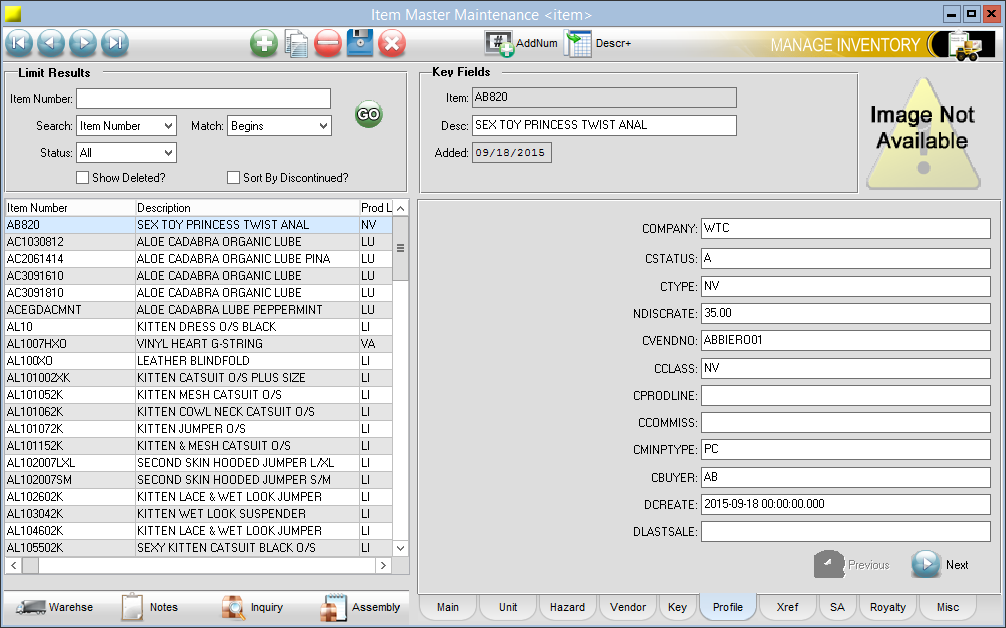
\includegraphics[width=\textwidth]{../img/image60}
		\caption{ITEM Item Master Maintenance Profile Tab}
	\end{figure}
	\item Profile Tab\\
	60 additional fields to rename and use as you want. Able to print on forms and reports.
	\begin{figure}[H]
		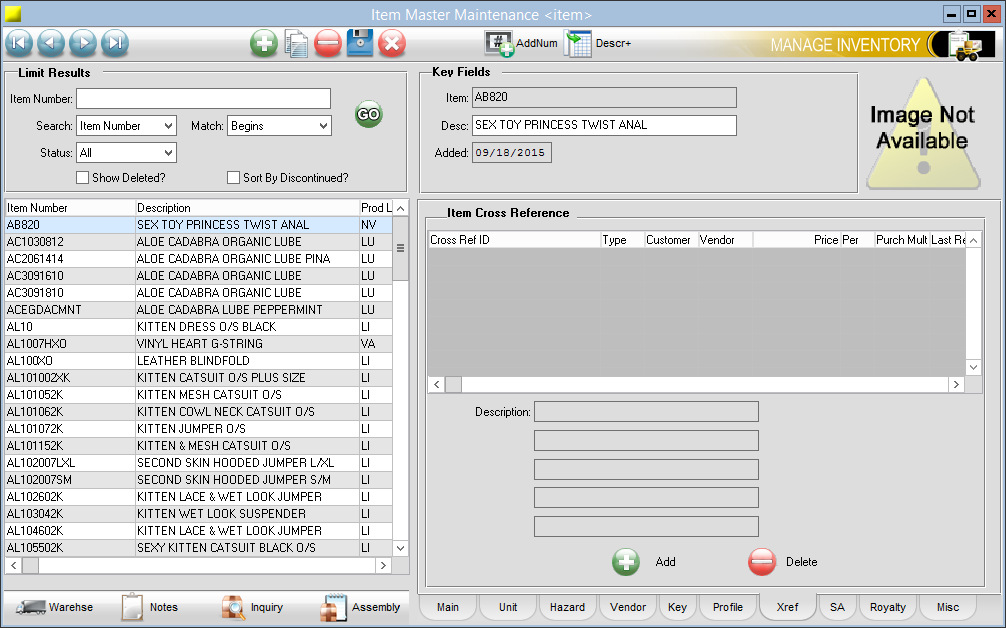
\includegraphics[width=\textwidth]{../img/image61}
		\caption{ITEM Item Master Maintenance Xref Tab}
	\end{figure}
	\item Xref Tab \textemdash To identify the item by using a different name or number that is not your main part number
	\begin{itemize}
		\item Cross Ref ID \textemdash Enter cross reference ID
		\item Type \textemdash Enter a number or code to identify type (optional), setup in \texttt{ITXFRTM}
		\item Customer \textemdash Account Number (optional)
		\item Vendor \textemdash Vendor Number (optional)
		\item Price \textemdash Fixed sell price (optional)
	\end{itemize}
\end{enumerate}

\subsubsection{Warehouse Item Maintenance}

\index{ERP-One Commands!WAITM}

The \texttt{WAITM} command is used to access Warehouse Item Maintenance

\begin{enumerate}
	
	\begin{figure}[H]
		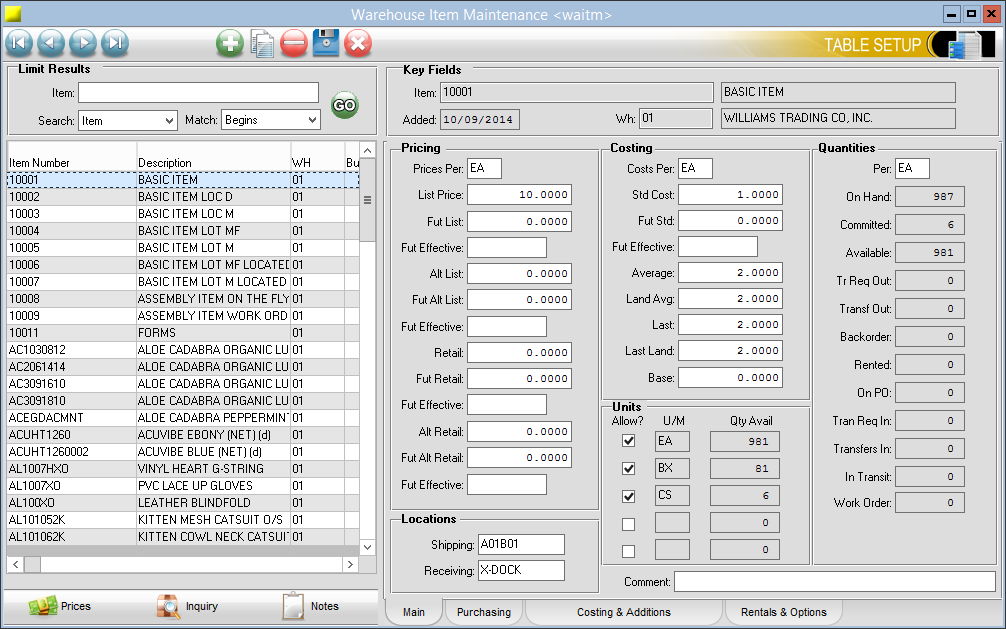
\includegraphics[width=\textwidth]{../img/image62}
		\caption{WAITM Warehouse Item Maintenance Main Tab}
	\end{figure}
	
	\item Main Tab
	\begin{itemize}
		\item Pricing \textemdash all options excluding Price Per are optional
		\begin{itemize}
			\item Price per \textemdash Enter E/M for List Price (required field)
			\item List Price \textemdash Enter list price
			\item Fut List \textemdash Enter a future list price
			\item Fut Effective \textemdash Date of future list to activate
			\item Alt List \textemdash Enter an alternate price
			\item Retail \textemdash Retail price
			\item Fut Retail \textemdash Future retail price
			\item Fut Effective \textemdash Date of future price to activate
			\item Alt Retail \textemdash Alternate retail price
		\end{itemize}
		\item Costing \textemdash used for PO's and costing for sales orders
		\begin{itemize}
			\item Manually Maintained
			\begin{itemize}
				\item Cost Per \textemdash U/M for cost price (required field)
				\item Std Cost \textemdash Standard Cost
				\item Fut Std \textemdash Future Standard Cost
				\item Fut Effective \textemdash Date of future standard cost to activate
				\item Base \textemdash Base Cost				
			\end{itemize}
			\item Auto Adjusted
			\begin{itemize}
				\item Average \textemdash Average Cost
				\item Land Avg. \textemdash Landed Average Cost
				\item Last \textemdash Last Cost
				\item Last Land \textemdash Last Landed Cost
			\end{itemize}
		\end{itemize}
		\item Quantities
		\begin{itemize}
			\item Per \textemdash U/M that On Hand and Committed Quantities are based on
			\item On Hand \textemdash Quantity of the item in the system
			\item Committed \textemdash Quantity committed to order but not processed yet
			\item Available \textemdash Quantity that are not committed to an order
			\item Backorder \textemdash How many are on back order
			\item On PO \textemdash How many are on a purchase order
		\end{itemize}
		\item Allow
		\begin{itemize}
			\item U/M \textemdash Determines what U/M is allowed for item
			\item Qty. Available \textemdash How many are available for the U/M
		\end{itemize}
		\item Locations \textemdash Generic or default locations for warehouse item
		\begin{itemize}
			\item Shipping \textemdash Location to ship from
			\item Receiving \textemdash Location for receiving
		\end{itemize}
	\end{itemize}
		
	\begin{figure}[H]
		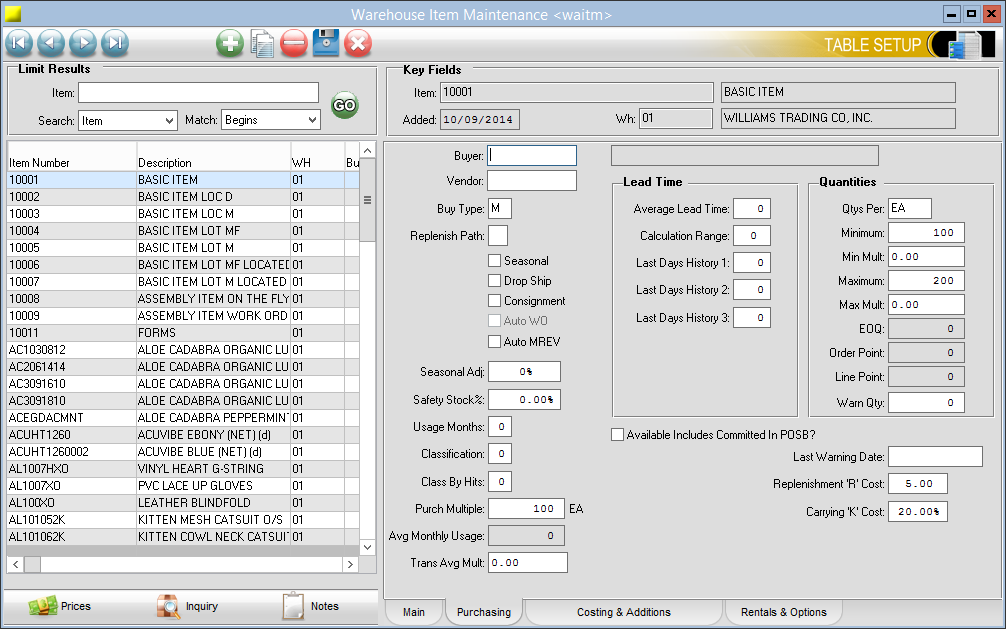
\includegraphics[width=\textwidth]{../img/image63}
		\caption{WAITM Warehouse Item Maintenance Purchasing Tab}
	\end{figure}
		
	\item Purchasing Tab
	\begin{itemize}
		\item Buy Type \textemdash The 'Suggested Buy' type indicates the method used to calculate a suggested quantity to reorder for a warehouse item.
		\begin{itemize}
			\item E \textemdash Economic Order Quantity method
			\item C \textemdash Item Usage Classification method
			\item M \textemdash Minimum / Maximum calculation method
			\item H \textemdash Hits default setting to determine replenishment
		\end{itemize}
		\item Purch Multiple \textemdash Increments for purchasing
		\item Lead Time\\
		Average lead Time \textemdash Calculated average time to receive item into stock after ordering (see \texttt{ITRPU} and \texttt{ITRPM} instructions)		
		\item Quantities \textemdash Settings for Buy Type
		\begin{itemize}
			\item Qtys. Per \textemdash U/M for stock
			\item M \textemdash Minimum / Maximum calculation method drives:
			\begin{itemize}
				\item Minimum \textemdash Minimum to keep in stock
				\item Maximum \textemdash Maximum to keep in stock
			\end{itemize}
			\item E \textemdash Economic Order Quantity method drives:
			\begin{itemize}
				\item EOQ
				\item Order Point
				\item Line Point
			\end{itemize}
			\item Warn Qty. \textemdash Optional, when item falls below this quantity, will receive a pop-up warning in Order Entry. \texttt{XO} option named "wa\_disp\_qty\_warn\_msg" must be set to "Yes" to activate
		\end{itemize}
	\end{itemize}
	
	\begin{figure}[H]
		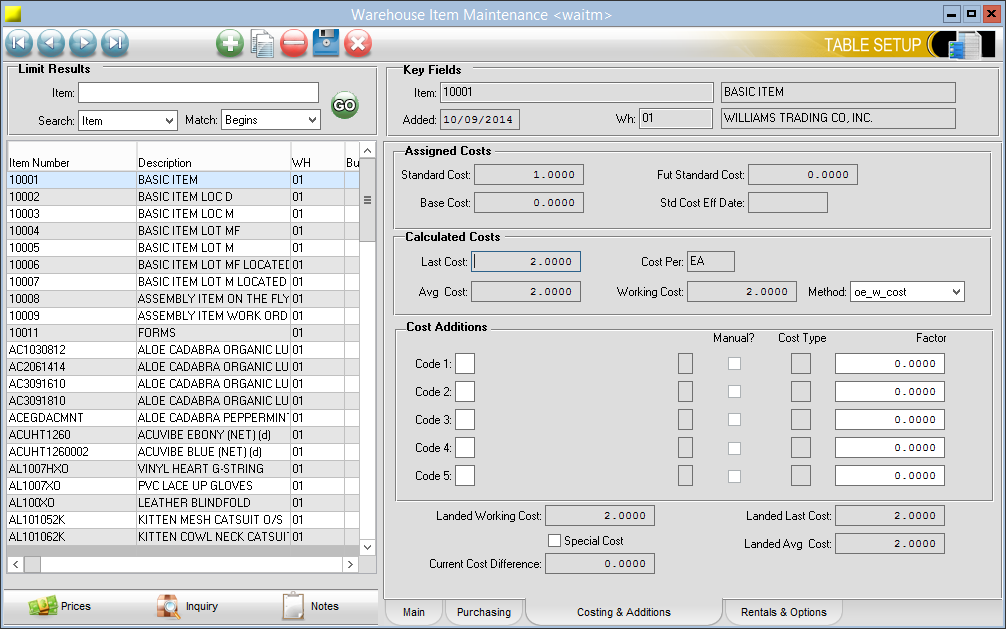
\includegraphics[width=\textwidth]{../img/image64}
		\caption{WAITM Warehouse Item Maintenance Costing \& Additions Tab}
	\end{figure}
	
	\item Costing and Additions Tab\\
	Setup in \texttt{POACM} affects landed costs
	\begin{itemize}
		\item Cost Additions \textemdash Codes 1-5 \textemdash Default add on's for item per warehouse
	\end{itemize}
	
	\begin{figure}[H]
		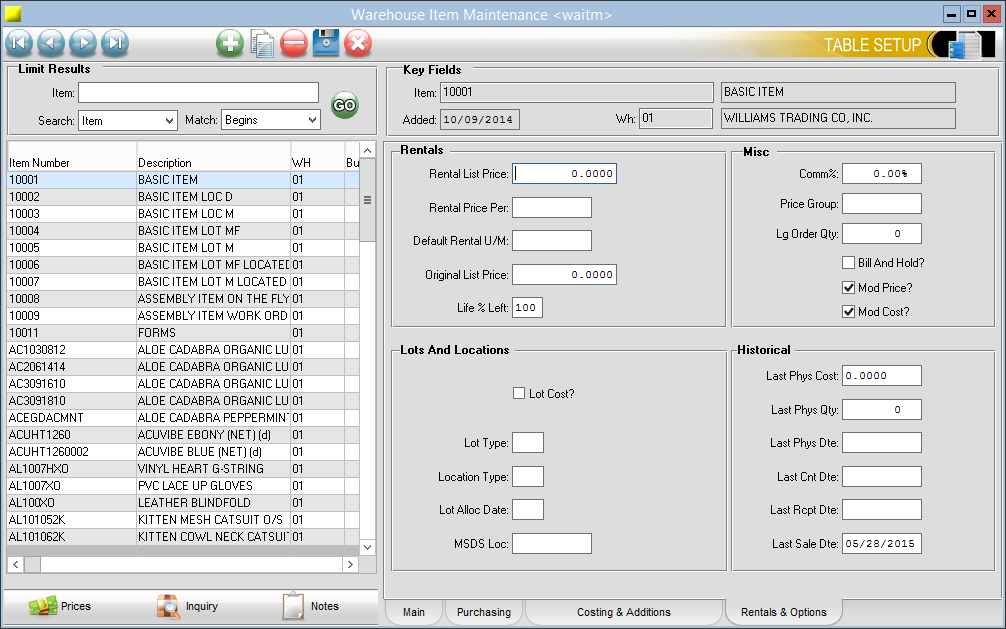
\includegraphics[width=\textwidth]{../img/image65}
		\caption{WAITM Warehouse Item Maintenance Rentals and Options Tab}
	\end{figure}
	
	\item Rentals and Options Tab
	\begin{itemize}
		\item If lot and located table is set to WA\_ITEM in \texttt{XO} called "lot\_loc\_setup", use the fields on this tab to indicate lot and / or location type and lot cost.
		\item Set the rental information if the item in this warehouse is rented out to customers
	\end{itemize}
\end{enumerate}

\subsubsection{Item Notes Maintenance}

\index{ERP-One Commands!ITNM}

The \texttt{ITNM} command is used to access Item Notes Maintenance

\begin{figure}[H]
	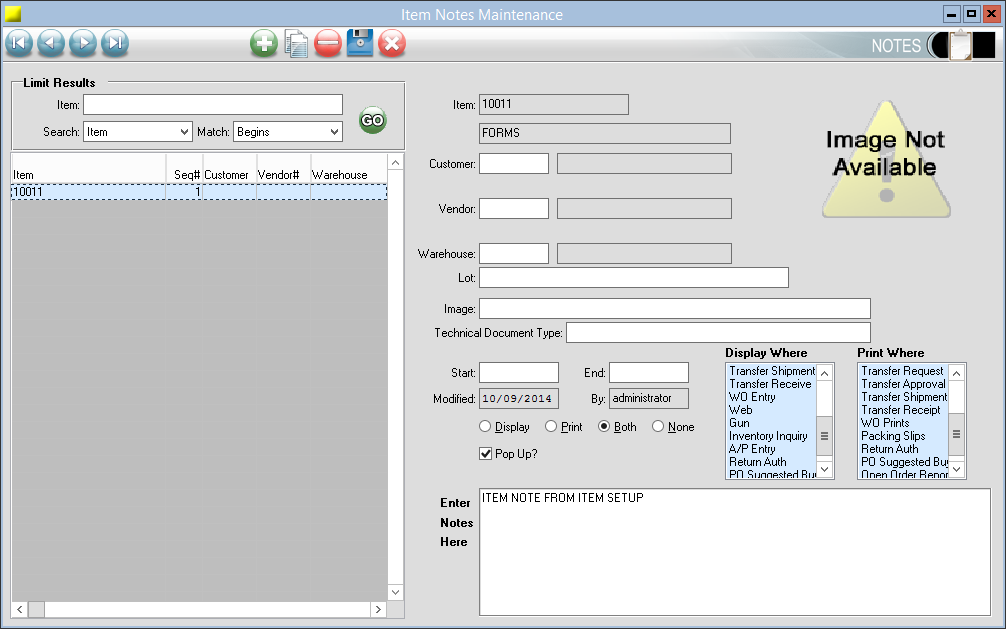
\includegraphics[width=\textwidth]{../img/image66}
	\caption{ITNM Item Notes Maintenance}
\end{figure}

You can set a note at item level. Notes can also be entered in at time of order entry or purchase order entry, per order or line item. Within notes, you have options on where, when, and what you would like it to print on. You can choose for it to be a pop up and / or display. You may also have an expiration date of when you no longer want the note to be active.

\subsection{Vendor Maintenance}

\subsubsection{Vendor Master Maintenance}

\index{ERP-One Commands!VEMM}

The \texttt{VEMM} command is used to access Vendor Master Maintenance

\begin{enumerate}
	
	\begin{figure}[H]
		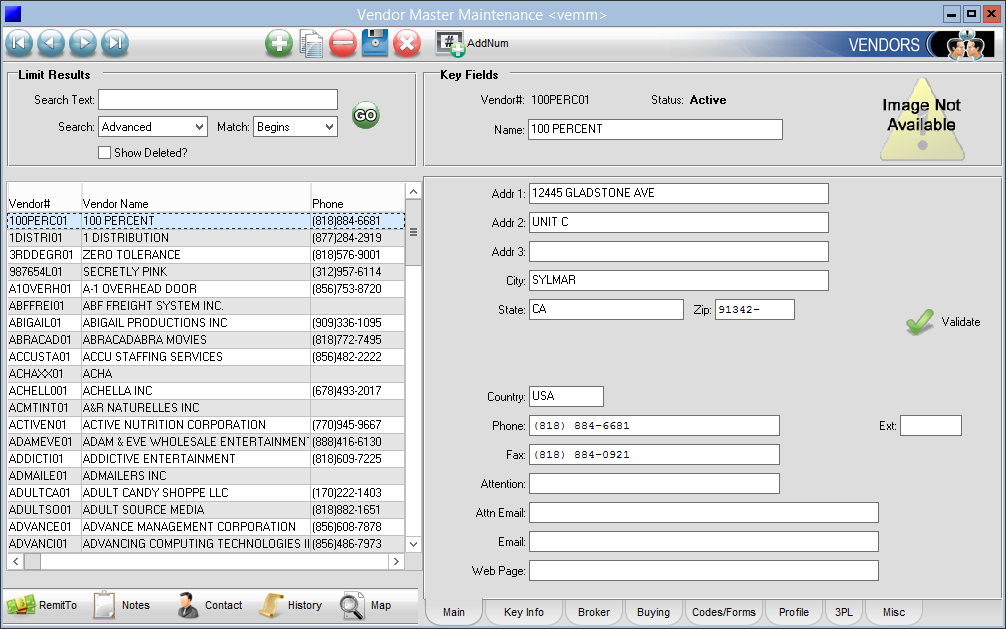
\includegraphics[width=\textwidth]{../img/image67}
		\caption{VEMM Vendor Master Maintenance Main Tab}
	\end{figure}
	
	\item Main Tab \textemdash This is where the core data for the vendor is stored. It will default into the puchase order entry screen and may be overridden as the PO is created
	\begin{itemize}
		\item Vendor Account Number Field \textemdash In this field you will add a unique vendor ID (numbers and letters allowed.) The ID can not be duplicated.
		\item Name \textemdash Enter vendor name
		\item Country \textemdash Based upon country codes, dictates how the address screen is laid out. Using F1 in this field opens a list of country codes.
		\item Address \textemdash Address 1 is the main address
		\item Attention \textemdash Primary contact
		\item Attention Email \textemdash Primary email address
		\item Email \textemdash Primary email for vendor
		\item Webpage \textemdash Vendor's web page		
	\end{itemize}	
	
	\begin{figure}[H]
		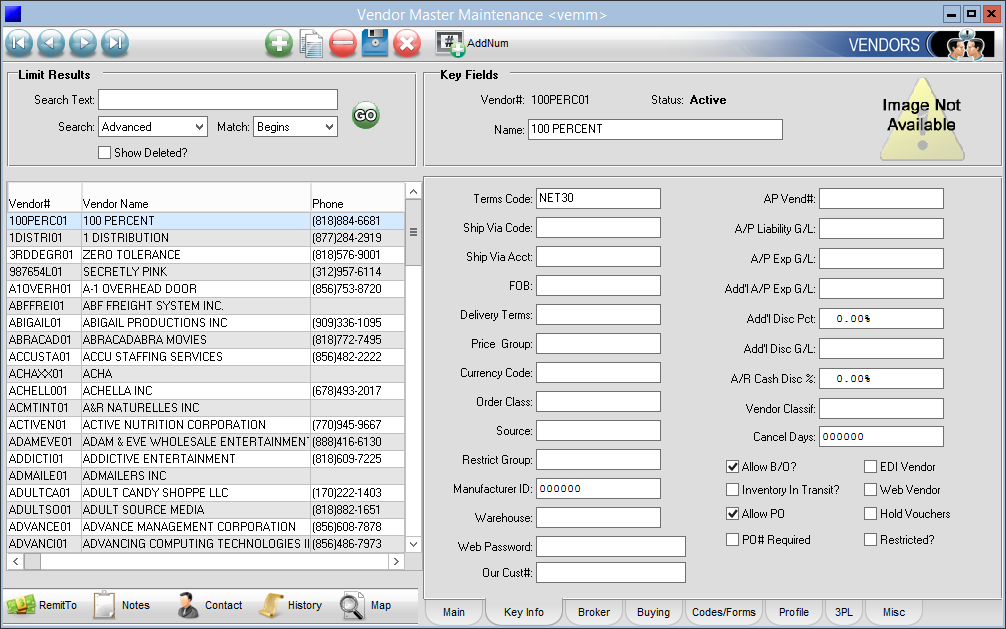
\includegraphics[width=\textwidth]{../img/image68}
		\caption{VEMM Vendor Master Maintenance Key Info Tab}
	\end{figure}
	
	\item Key Info Tab
	\begin{itemize}
		\item Terms Code \textemdash Terms with vendor, using F1 will bring up \texttt{SYTCM}
		\item Ship Via Code \textemdash Default how you want product shipped to you, can be overridden at purchase order entry. Using F1 in this field will bring up \texttt{SYSVM}. May print on purchase order.
		\item Ship Via Acct \textemdash Your account number with shipping company for collect, prints on purchase order.
		\item Currency Code \textemdash Using F1 in this field will bring up currency options \texttt{SYCRM}
		\item Web Password \textemdash Store password for vendor website
		\item Our Customer \# \textemdash Your customer number with the vendor
		\item A/P Liability G/L \textemdash Optional override of default A/P account
		\item A/P Exp G/L \textemdash Inventory GL / Utility GL for vendor
		\item Add'l A/P Exp. G/L \textemdash Typically freight in GL (These are default GL for AP Vouchers)
	\end{itemize}
	
	\begin{figure}[H]
		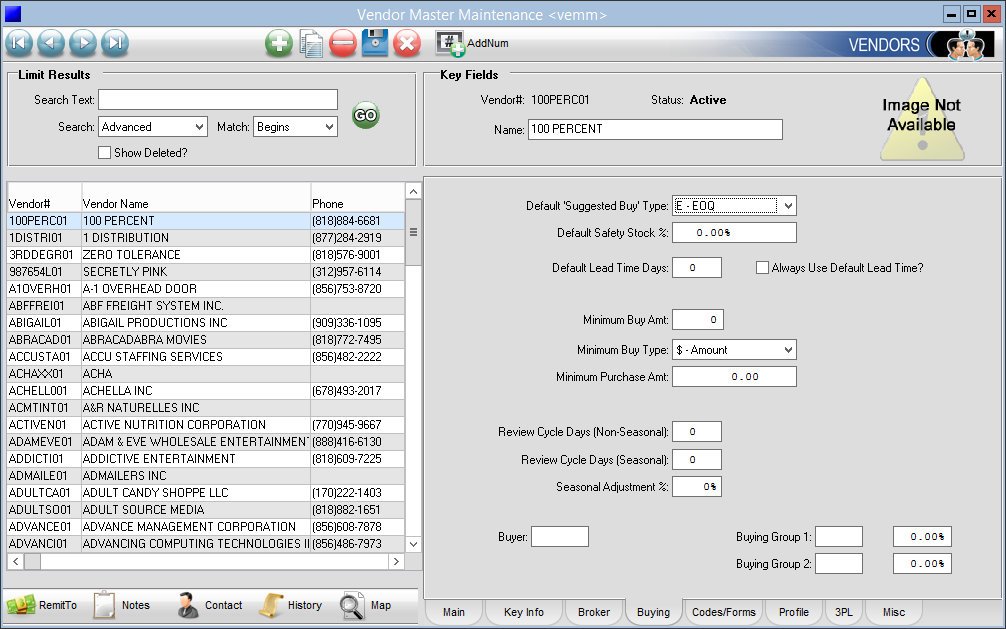
\includegraphics[width=\textwidth]{../img/image69}
		\caption{VEMM Vendor Master Maintenance Buying Tab}
	\end{figure}
	
	\item Buying Tab \textemdash Default setting for purchasing
	\begin{itemize}
		\item Minimum Buy Amount \textemdash How much in amount or weight, based on buy type
		\item Minimum Buy Type \textemdash Purchase requirements, in amount or weight, based on buy type, the above MIN/MAX work together
		\item Minimum Purchase Amount \textemdash If vendor requires the purchase to reach a minimum buy amount. If you don't meet the criteria upon accepting the purchase order, you will get a pop up warning, but the order can still be placed
	\end{itemize}
	
	\begin{figure}[H]
		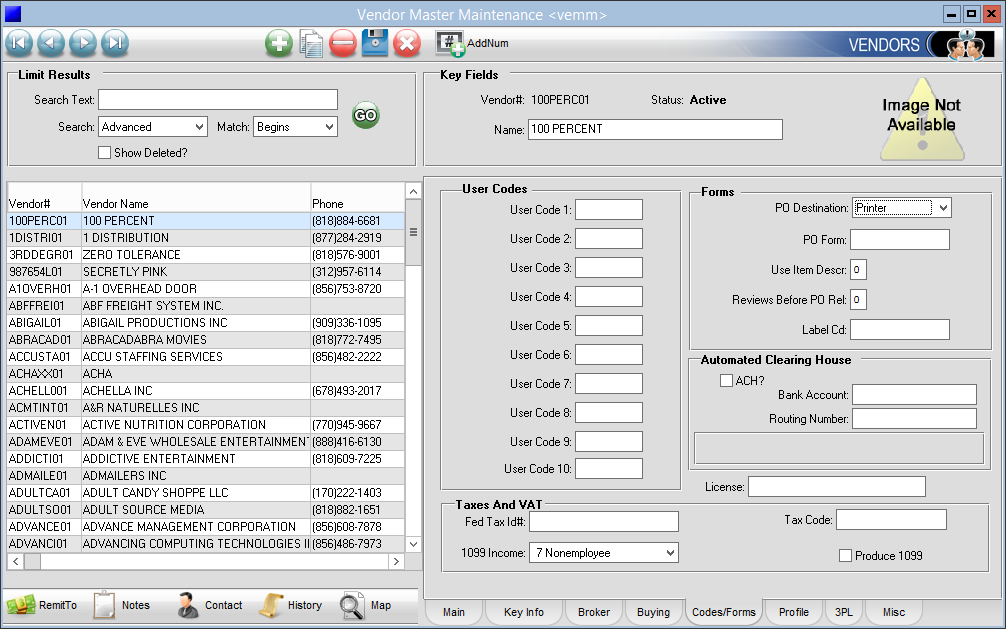
\includegraphics[width=\textwidth]{../img/image70}
		\caption{VEMM Vendor Master Codes / Forms Tab}
	\end{figure}
	
	\item Codes / Forms Tab
	\begin{itemize}
		\item User Codes \textemdash Ten user codes to use any way you want for reporting purposes. Option to print on documents.
		\item Forms
		\begin{itemize}
			\item PO Destination \textemdash Default setting for how you want the purchase order to print, email or fax.			
		\end{itemize}
		\item Taxes and VAT
		\begin{itemize}
			\item If 1099 type vendor, check the option to produce 1099
		\end{itemize}
	\end{itemize}
	
	\begin{figure}[H]
		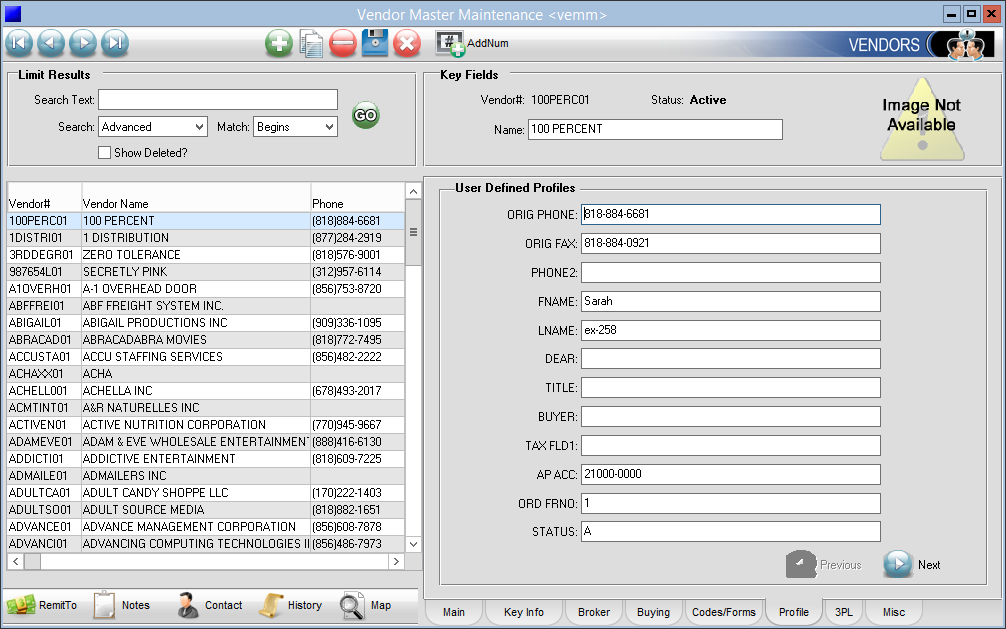
\includegraphics[width=\textwidth]{../img/image71}
		\caption{VEMM Vendor Master Profile Tab}
	\end{figure}
	
	\item Profile Tab
	\begin{itemize}
		\item Profile Info \textemdash Sixty additional fields you can label in \texttt{SYPROF} and create F1 lookup tables in \texttt{VEPF1}
	\end{itemize}
\end{enumerate}

\subsubsection{Vendor Remit To Maintenance}

\index{ERP-One Commands!VEREM}

The \texttt{VEREM} command is used to access Vendor Remit To Maintenance.

\begin{figure}[H]
	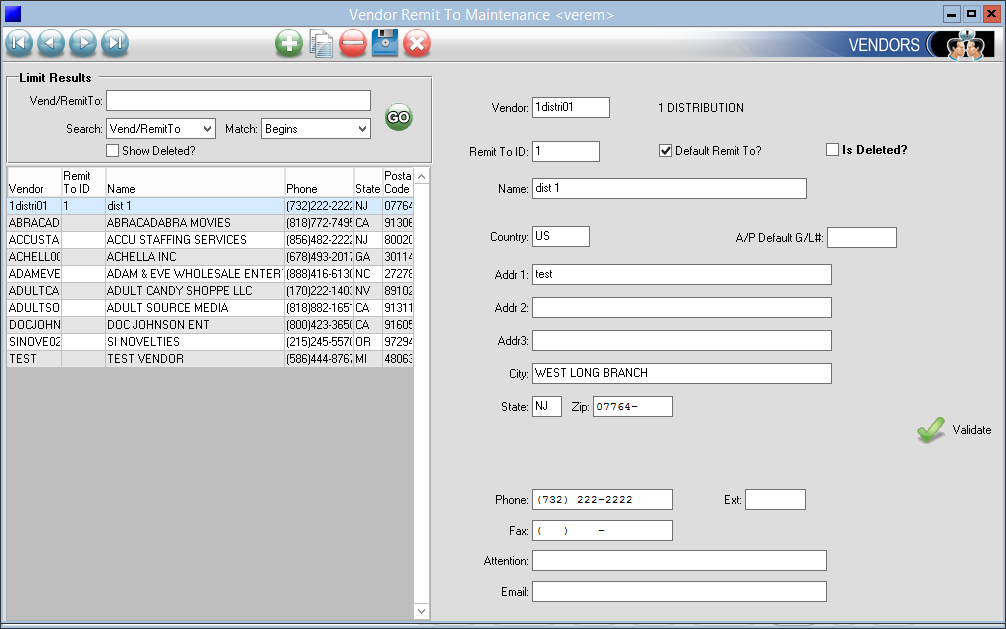
\includegraphics[width=\textwidth]{../img/image72}
	\caption{VEREM Vendor Remit To Maintenance}
\end{figure}

\begin{itemize}
	\item To add a new remit to, click on the add button. This opens up the Remit to ID.
	\item Remit to ID \textemdash In this field you will add a unique ID (numbers and letters allowed.) The ID can not be duplicated.
	\item Name \textemdash Enter Remit To name
	\item Country \textemdash Required field. Country code determines how the address screen is paied out. Use F1 to find country code.
	\item Address \textemdash Address 1 is the Remit To address for payments
	\item Phone / Fax \textemdash Remit To phone and fax
	\item Attention \textemdash Remit To contact
	\item Email \textemdash Remit To Email Address
	\item Webpage \textemdash Vendor's web page
	\item After you have completed your data entry, click save
\end{itemize}

\subsubsection{Vendor Master Maintenance Notes}

\index{ERP-One Commands!VENM}

The \texttt{VENM} command is used to access Vendor Notes Maintenance.

\begin{figure}[H]
	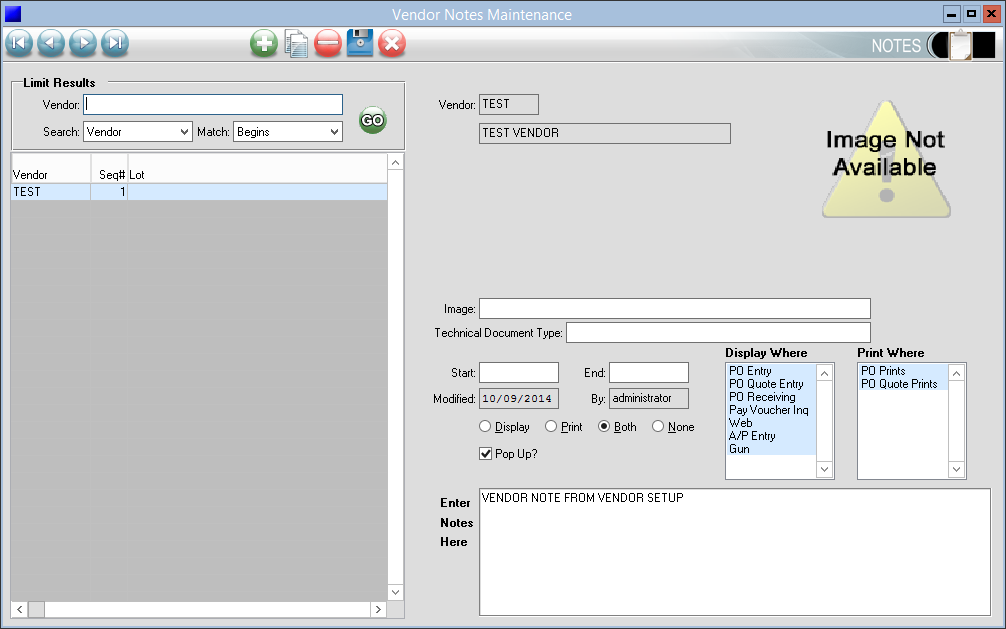
\includegraphics[width=\textwidth]{../img/image73}
	\caption{VENM Vendor Master Maintenance Notes}
\end{figure}

You can create a note at the vendor level. Notes can also be entered in at time of purchase order entry, per order or line item. Within notes, you have options as to where the note will display in ERP One and on what forms you would like it to print. You can choose for it to be a pop up and / or display. You may also have an expiration date for when you no longer want that note to be active.

\subsubsection{Vendor Contacts Maintenance}

\index{ERP-One Commands!VECOM}

The \texttt{VECOM} command is used to access Vendor Contacts Maintenance.

\begin{figure}[H]
	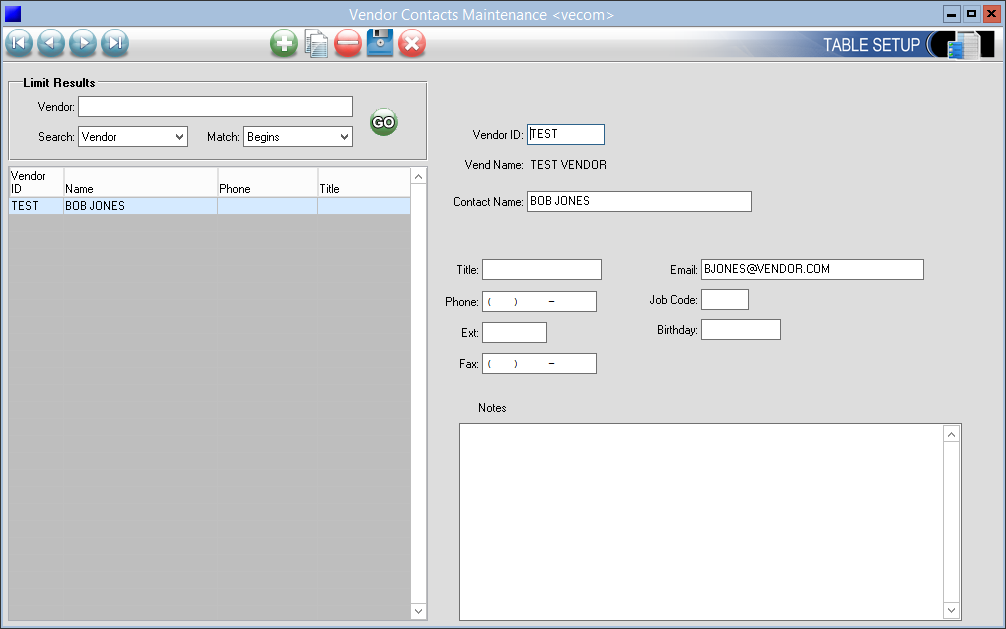
\includegraphics[width=\textwidth]{../img/image74}
	\caption{VENM Vendor Master Maintenance Notes}
\end{figure}

Vendor contacts can be added during vendor set up and can be added during purchase order entry. To add in purchase order entry, while in the header screen, hover over the Vendor Contact on the left. A clickable button appears, which you can click on and enter contact information then click Save. The next time you are placing an order you can use F1 in that field and bring up the saved contacts.

\subsection{Customer Maintenance}

\subsubsection{Customer Master Maintenance}

\index{ERP-One Commands!CUMM}

The \texttt{CUMM} command is used to access Customer Master Maintenance.

\begin{enumerate}
	
	\begin{figure}[H]
		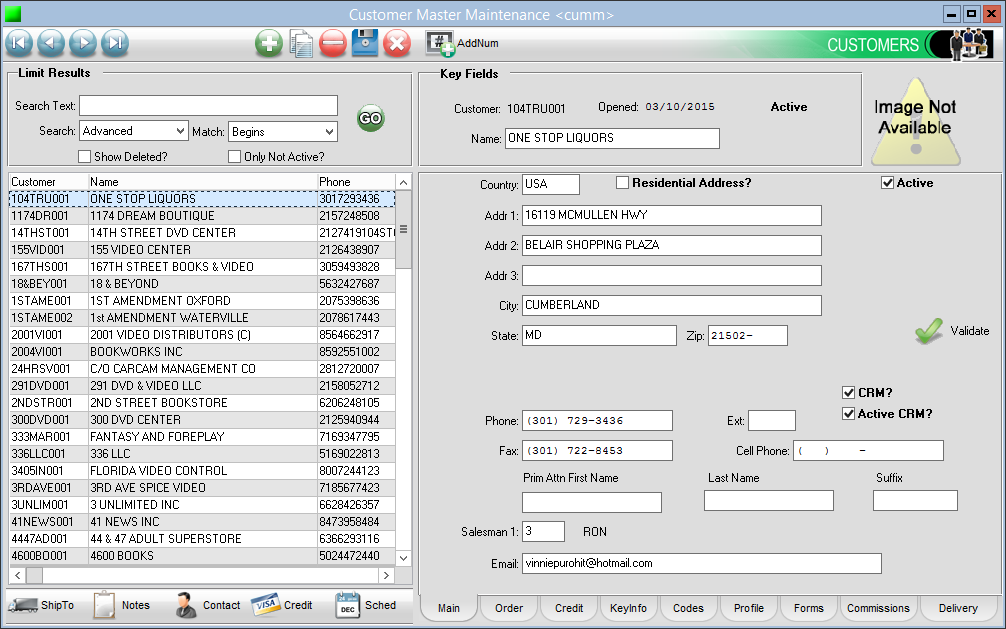
\includegraphics[width=\textwidth]{../img/image75}
		\caption{CUMM Customer Master Maintenance Main Tab}
	\end{figure}
	
	\item Main Tab \textemdash This is where all the core data for the customer is stored. The data that is stored for the customer will default into the order entry screen when placing an order. Default data can be overridden in order entry.
	\begin{itemize}
		\item Customer Field \textemdash In this field you will add a unique customer ID, (nummbers and letters allowed.) The ID can not be duplicated.
		\item Name \textemdash Enter customer name
		\item Country \textemdash Based upon Country Code, dictates how the address screen is laid out. Using F1 in this field opens a list of countries. Choose country by double clicking and then clicking Enter.
		\item Address \textemdash Address 1 is the true address.
		\item Map \textemdash Linked to Yahoo! maps.
		\item Active \textemdash If checked, customer is active
		\item Phone / Fax \textemdash Enter main number for customer
		\item Prime Attn. \textemdash Enter primary contact for customer
		\item Salesman 1 \textemdash Required field. Using F1 in this field opens up a list of sales people.
		\item Email \textemdash Enter primary email contact
	\end{itemize}
	
	\begin{figure}[H]
		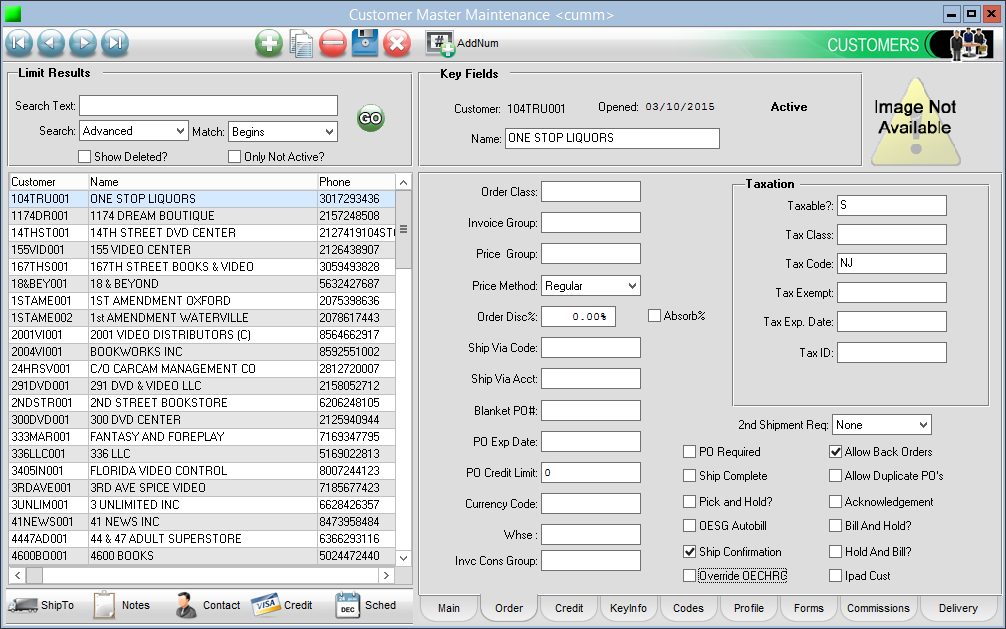
\includegraphics[width=\textwidth]{../img/image76}
		\caption{CUMM Customer Master Maintenance Order Tab}
	\end{figure}
	
	\item Order Tab \textemdash Set certain criteria of how the customer wants their orders handled.
	\begin{itemize}
		\item Ship Via Code \textemdash The way the order ships from the warehouse to the customer. Use F1 to access \texttt{SYSVM} for the options of shipping codes
		\item Ship Via Acct \textemdash Enter customer shipping account if required
		\item Taxation (Per Order or Line Item)
		\begin{itemize}
			\item Taxable \textemdash Required field. This is how the customer will be taxed. Using F1 will display the following options:
			\begin{itemize}
				\item Always \textemdash Customer is always taxed
				\item Never \textemdash Customer is never taxed (Tax Code required)
				\item Sometimes \textemdash Whether order is taxed is prompted for at order entry
			\end{itemize}
			\item Tax Code \textemdash Required field. Set up percentages of the tax according to state, country, jurisdictions etc.. Using F1 in this field will open \texttt{CUTXM}
			\item Tax Exempt \textemdash If customer is tax exempt, you can store the tax exempt number in this field
			\item Tax Exempt Date \textemdash Tax exempt number expiration date is displayed in order entry
		\end{itemize}
		\item Checked
		\begin{itemize}
			\item PO Required \textemdash Require a PO before you are able to leave the header screen in Order Entry
			\item Ship Complete \textemdash ERP One allocates the items in stock, will not print or prompt to print pick ticket until the order is 100% complete
			\item Pick and Hold \textemdash ERP One allocates the items, will print pick ticket and items will be put in a staging area until order is completed
			\item $2^{nd}$ Shipment Req \textemdash you have options also for a second shipment, to ship complete or pick and hold
			\item Allow Back Orders \textemdash If checked, allows back orders, unchecked will consider the order complete and not backorder items
			\item Allow Duplicate PO's \textemdash If checked will PO numbers to be used more than once
			\item Acknowledgment \textemdash If checked, allows an acknowledgment to print for the customer
		\end{itemize}
	\end{itemize}
	
	\begin{figure}[H]
		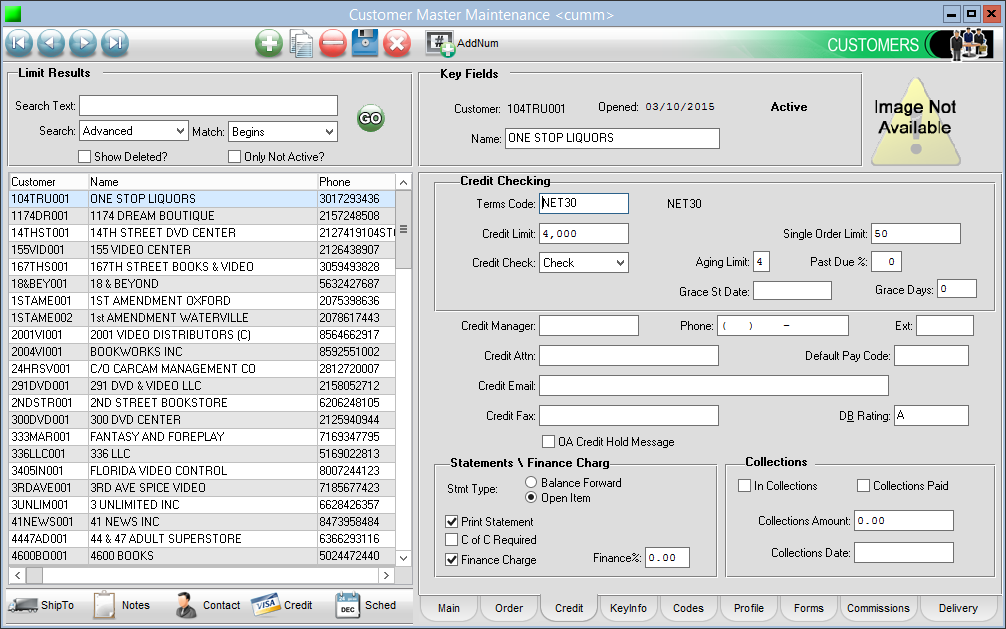
\includegraphics[width=\textwidth]{../img/image77}
		\caption{CUMM Customer Master Maintenance Credit Tab}
	\end{figure}
	
	\item Credit Tab
	\begin{itemize}
		\item Terms Code \textemdash Payment terms with customer, drives invoice aging and discount on AR side for cash receipts. Using F1 in this field will bring up \texttt{SYTCM}
		\item Credit Limit \textemdash Dollar amount for credit limit if credit is checked
		\item Credit Check
		\begin{itemize}
			\item Always Pass \textemdash Always pass order through, no credit check is done
			\item Check \textemdash Check for status of credit, verify dollar amount and aging
			\item Always Fail \textemdash Always put sales order on credit hold until released
		\end{itemize}
		\item Aging Limit (set by \texttt{XO} options)
		\begin{itemize}
			\item 1 \textemdash 30 days
			\item 2 \textemdash 60 days
			\item 3 \textemdash 90 days
			\item 4 \textemdash 120 days
			\item 5 \textemdash 150 days
		\end{itemize}
		\item Statement \ Finance Charge
		\begin{itemize}
			\item Print Statement \textemdash If checked, will allow an A/R statement to print for the customer
			\item C of C \textemdash If checked, option to print certification of compliance
		\end{itemize}
	\end{itemize}
	
	\begin{figure}[H]
		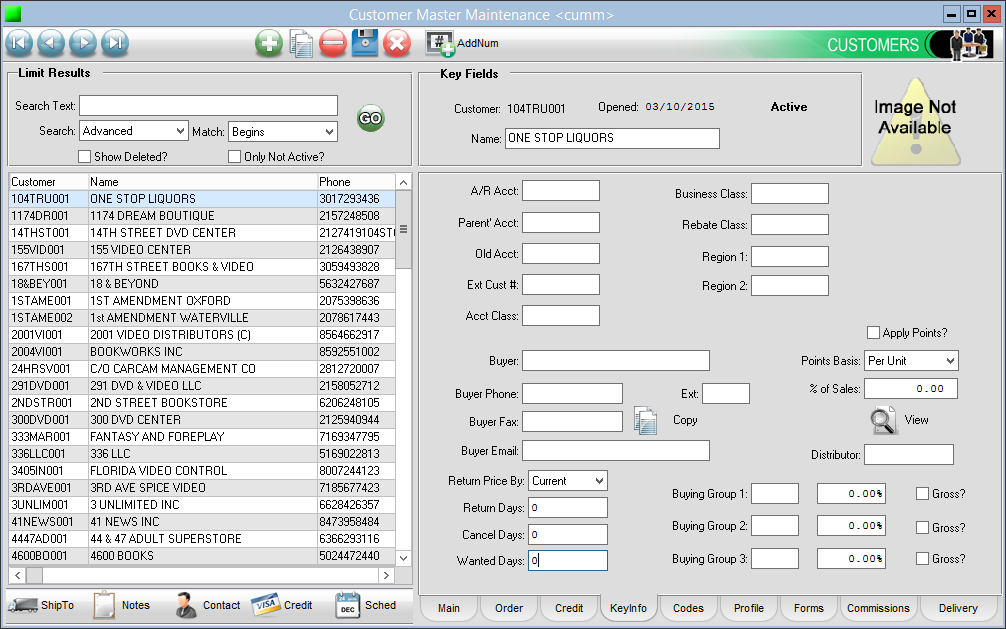
\includegraphics[width=\textwidth]{../img/image78}
		\caption{CUMM Customer Master Maintenance Key Info Tab}
	\end{figure}
	
	\item Key Info Tab
	\begin{itemize}
		\item A/R Acct \textemdash If multiple accounts are in ERP One, but need only one Bill To for cash receipts
		\item Parent' Acct \textemdash If the sales of one account should be reported in another
		\item Business Class \textemdash Selects reporting options, see \texttt{CUBC}
	\end{itemize}
	
	\begin{figure}[H]
		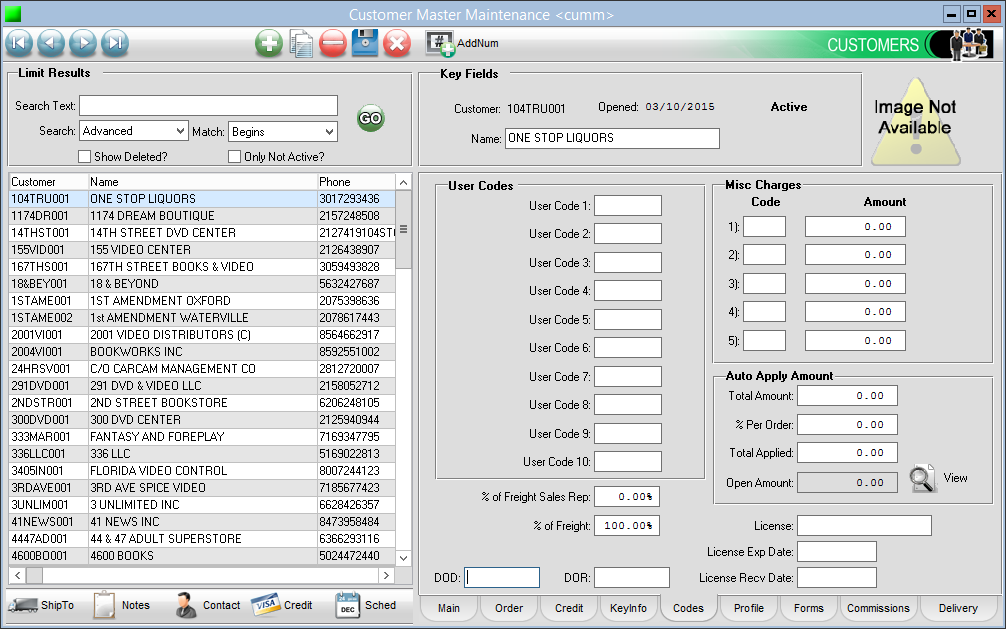
\includegraphics[width=\textwidth]{../img/image79}
		\caption{CUMM Customer Master Maintenance Codes Tab}
	\end{figure}
	
	\item Codes Tab
	\begin{itemize}
		\item User Codes \textemdash Ten user codes to use any way you want for reporting purposes. Option to print on documents.
		\item Misc. Charges
		\begin{itemize}
			\item Code \textemdash Establishes code for additional fee to always apply to customer's orders. Using F1 in this field will open up \texttt{OETCM}.
			\item Amount \textemdash Enter in the amount of additional fee
		\end{itemize}
	\end{itemize}
	
	\begin{figure}[H]
		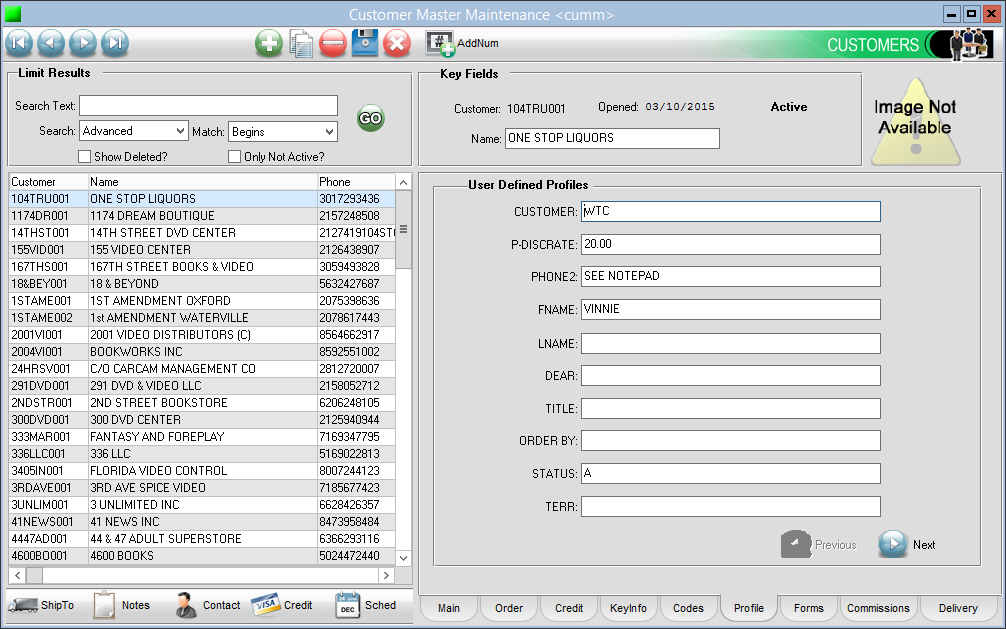
\includegraphics[width=\textwidth]{../img/image80}
		\caption{CUMM Customer Master Maintenance Profile Tab}
	\end{figure}
	
	\item Profile Tab\\
	Sixty additional fields to rename and use any way you want, also available to print on documents.
	
	\begin{figure}[H]
		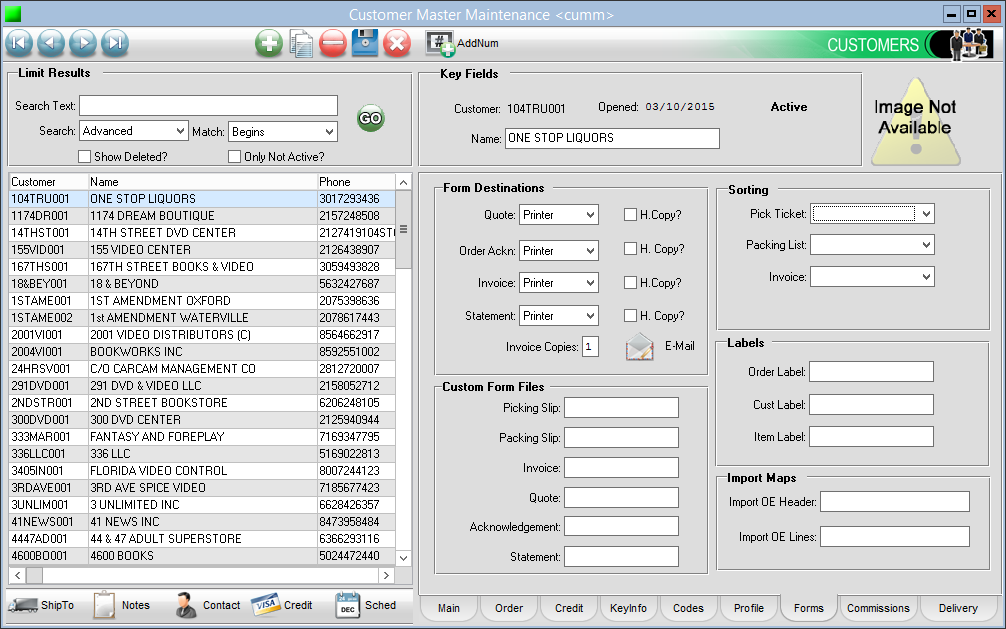
\includegraphics[width=\textwidth]{../img/image81}
		\caption{CUMM Customer Master Maintenance Forms Tab}
	\end{figure}
	
	\item Forms Tab
	\begin{itemize}
		\item Forms Destination \textemdash Set up the defaults on how the forms will be printed, emailed, or faxed to the customers
		\begin{itemize}
			\item Select option for the form
			\item Click Fax / Email Source to choose form
			\item H. Copy \textemdash If checked, hard copy will also be printed
		\end{itemize}
		\item Customer Forms \textemdash If a customer requires a different layout on their forms from the default, the alternative layout can be specified here
		\item Sorting \textemdash Choose specific sorting and printing options here
	\end{itemize}	
	
	\begin{figure}[H]
		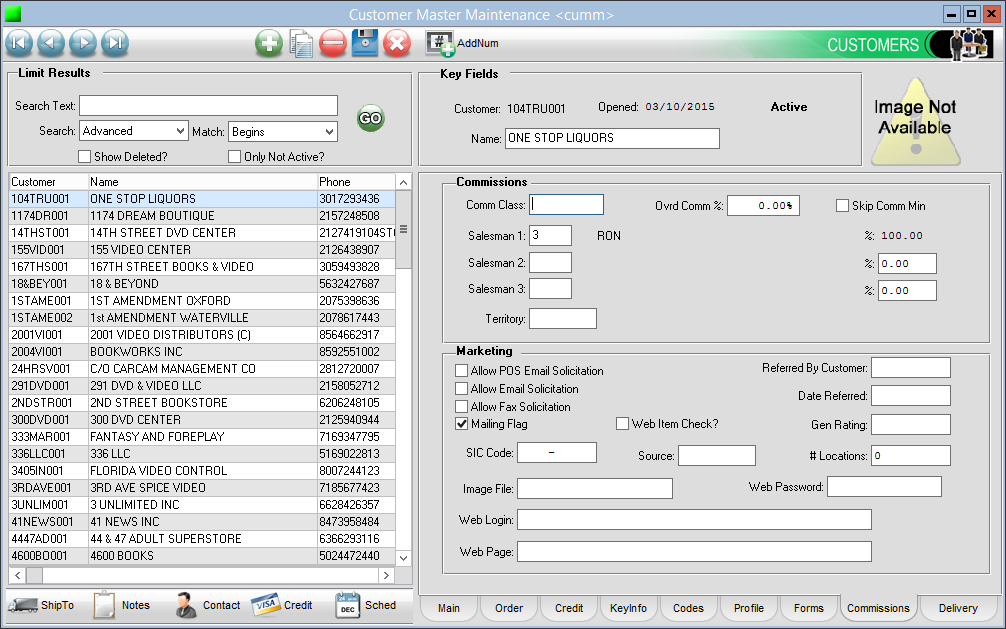
\includegraphics[width=\textwidth]{../img/image82}
		\caption{CUMM Customer Master Maintenance Commissions Tab}
	\end{figure}
	
	\item Commissions Tab
	\begin{itemize}
		\item Salesman 1 \textemdash Using F1 here will allow selecting sales person to receive commissions for this customer
		\item Salesman 2 \textemdash Optional field for split commissions
	\end{itemize}
\end{enumerate}

\subsubsection{Customer Ship To Maintenance}

\index{ERP-One Commands!CUSHM}

The \texttt{CUSHM} command is used to access Customer Ship To Maintenance.

\begin{enumerate}
	
	\begin{figure}[H]
		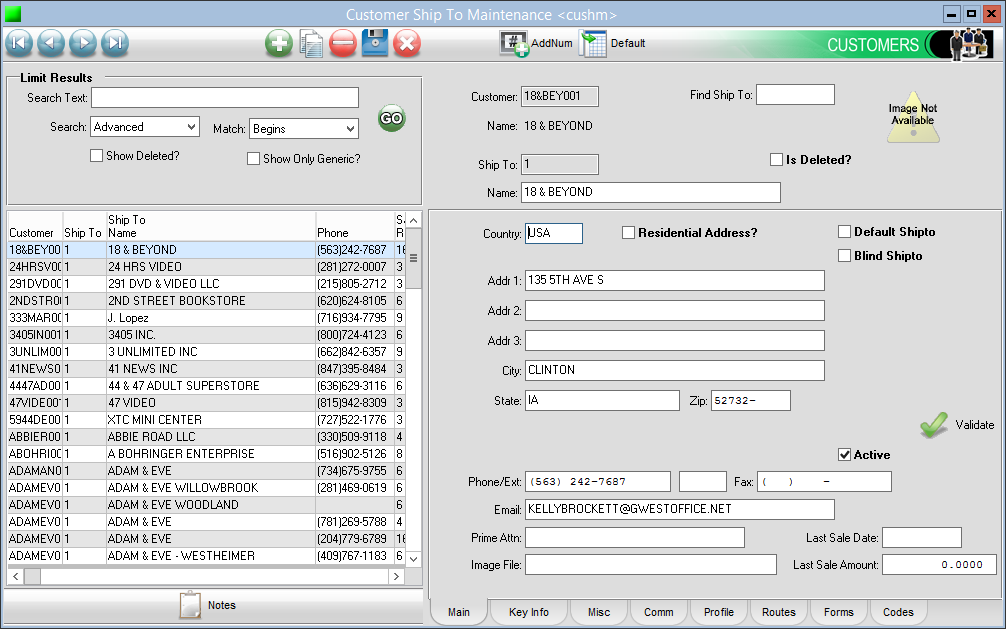
\includegraphics[width=\textwidth]{../img/image83}
		\caption{CUSHM Customer Ship To Maintenance Main Tab}
	\end{figure}
	
	\item Main Tab \textemdash This is where the core data for the customer ship to is stored. If a ship to is not set up that differs from the bill to, the bill to will auto generate into the ship to. Default data can be overridden at order entry time. You can have multiple ship to's.
	\begin{itemize}
		\item Ship to overrides Bill To
		\item Country \textemdash Uses country code, dictates how the address screen is laid out. Using F1 opens selection of country codes.
		\item Address1 \textemdash The address for ship to
		\item Map \textemdash Link to Yahoo! maps
		\item Phone / Fax \textemdash Main numbers for shipping address
		\item Email \textemdash Main email contact for shipping address
		\item Prime Attn \textemdash Primary contact for shipping address
	\end{itemize}
	
	\begin{figure}[H]
		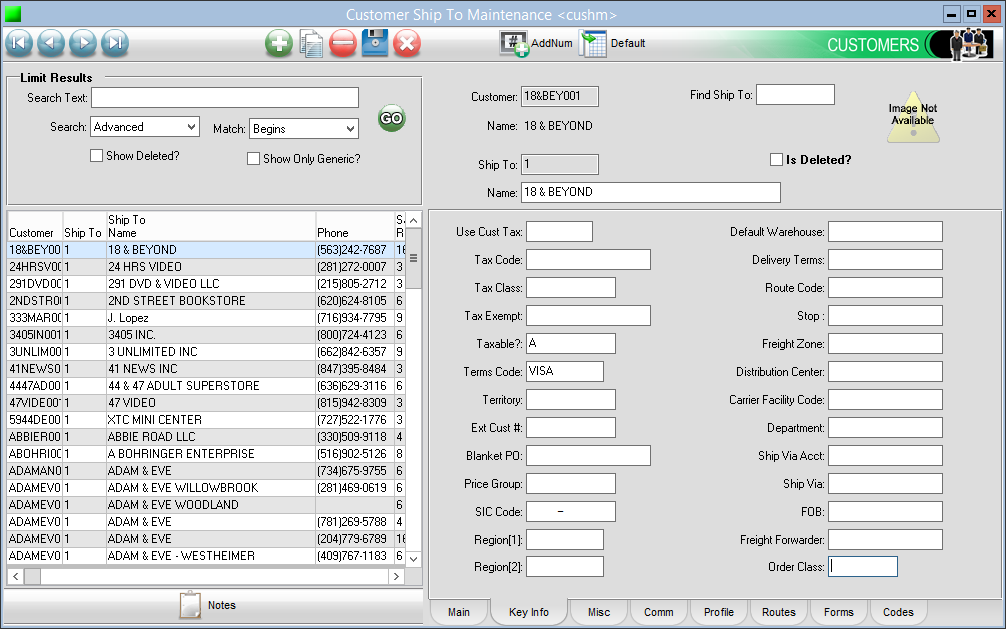
\includegraphics[width=\textwidth]{../img/image84}
		\caption{CUSHM Customer Ship To Maintenance Key Info Tab}
	\end{figure}
	
	\item Key Info Tab\\
	If your shipping terms are different from billing terms, add them here
	\begin{itemize}
		\item Tax
		\item Taxable
		\item Terms
		\item Ship Via
	\end{itemize}
	
	\begin{figure}[H]
		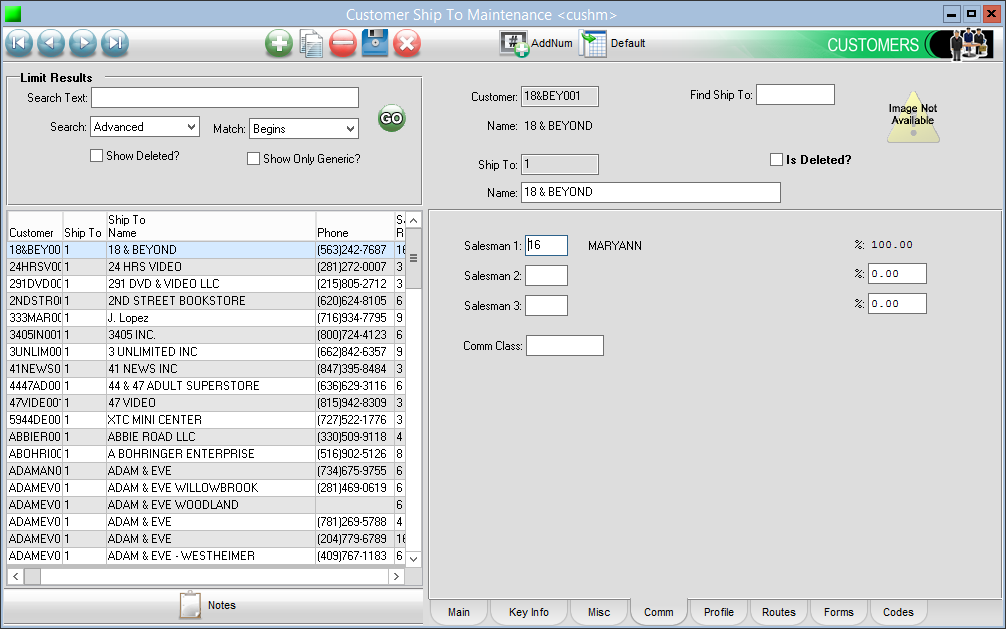
\includegraphics[width=\textwidth]{../img/image85}
		\caption{CUSHM Customer Ship To Maintenance Comm Tab}
	\end{figure}
	
	\item Comm Tab\\
	If commissions are based on ship to address, set up here
	
	\begin{figure}[H]
		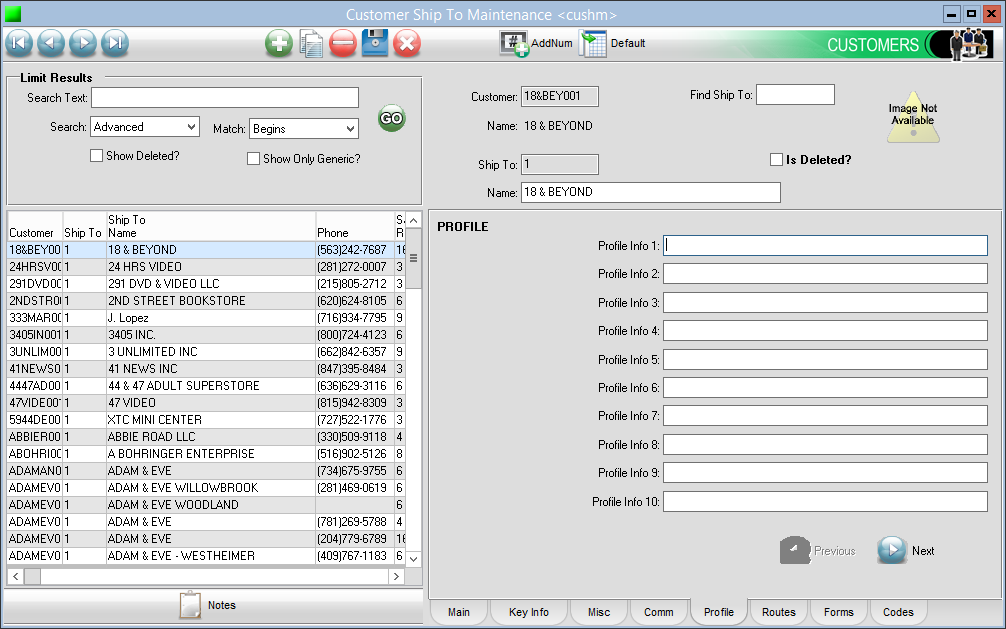
\includegraphics[width=\textwidth]{../img/image86}
		\caption{CUSHM Customer Ship To Maintenance Profile Tab}
	\end{figure}
	
	\item Profile Tab\\
	Sixty additional profile fields to rename and use any way. Option to print on documents.
	
	\begin{figure}[H]
		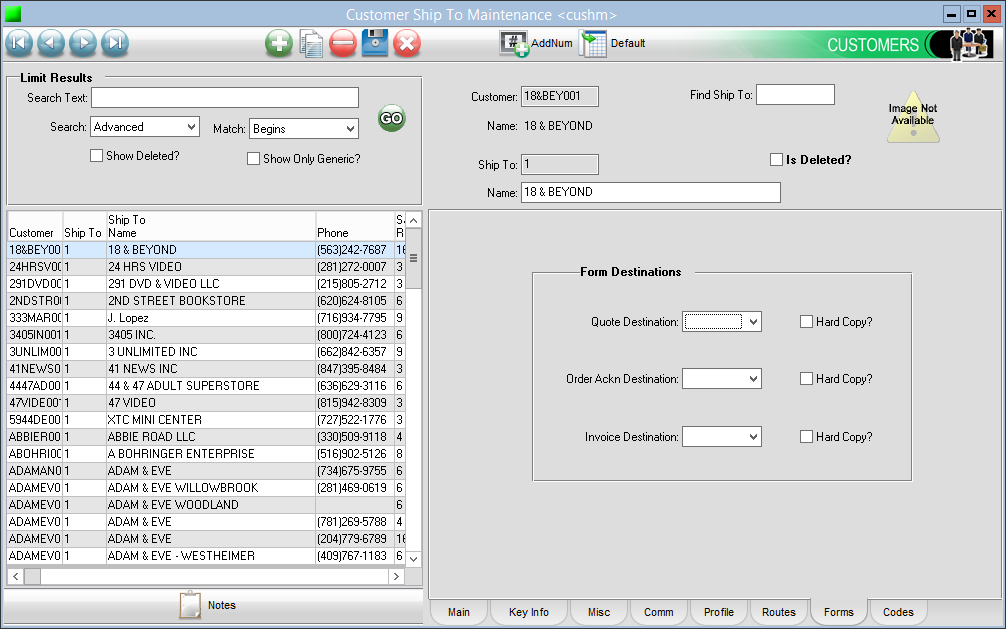
\includegraphics[width=\textwidth]{../img/image87}
		\caption{CUSHM Customer Ship To Maintenance Forms Tab}
	\end{figure}
	
	\item Forms Tab\\
	If you want to define how your forms are printed or sent based on the ship to
	
	\begin{figure}[H]
		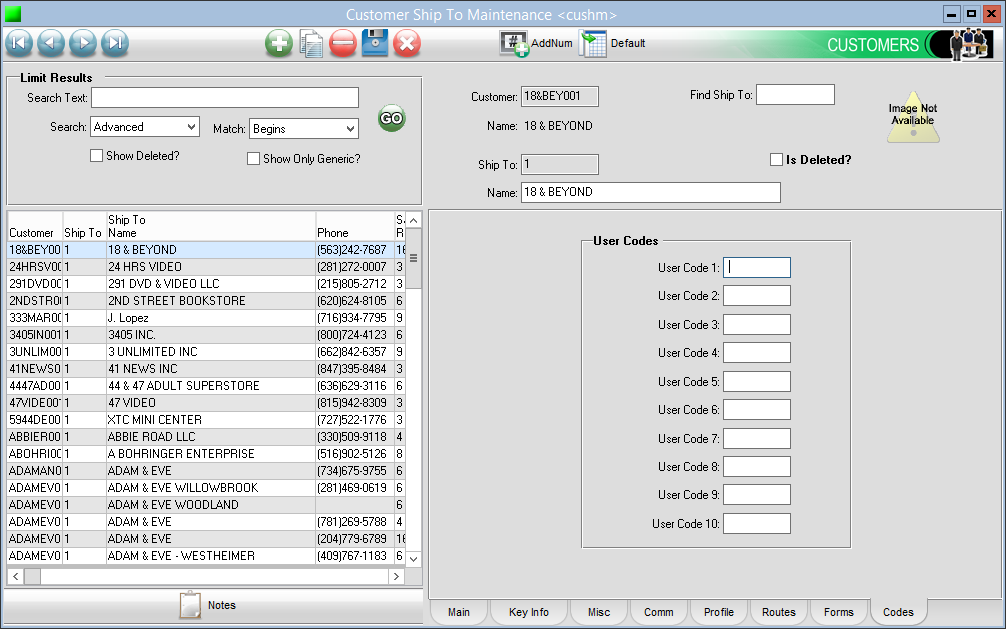
\includegraphics[width=\textwidth]{../img/image88}
		\caption{CUSHM Customer Ship To Maintenance Forms Tab}
	\end{figure}
	
	\item Codes Tab\\
	Ten additional codes to use any way, able to print on documents.
\end{enumerate}

\subsubsection{Customer Notes Maintenance}

\index{ERP-One Commands!CUNM}

The \texttt{CUNM} command is used to access Customer Notes Maintenance.

\begin{figure}[H]
	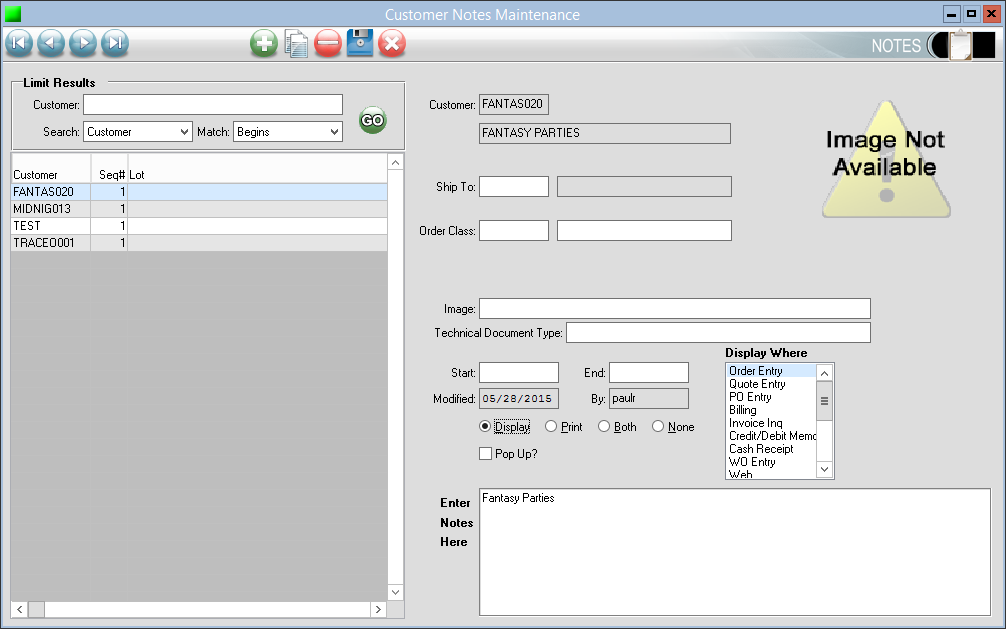
\includegraphics[width=\textwidth]{../img/image89}
	\caption{CUNM Customer Notes Maintenance}
\end{figure}

You can set a note at the customer level. Notes can also be entered at time of order entry per order or line item. Within notes, you have options on there and when to display the note, and what forms you would like it to print on. You can choose for it to be a pop up and / or display, also you may specify an expiration date for when you no longer want that note to be active.

\subsubsection{Customer Contacts Maintenance}

\index{ERP-One Commands!CUCOM}

The \texttt{CUCOM} command is used to access Customer Contacts Maintenance.

\begin{figure}[H]
	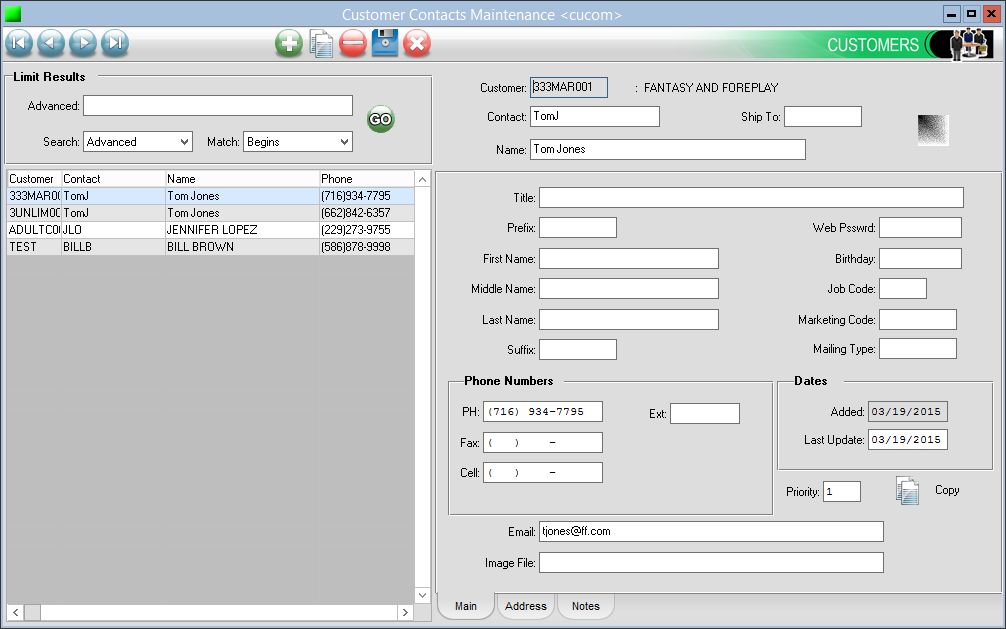
\includegraphics[width=\textwidth]{../img/image90}
	\caption{CUCOM Customer Contacts Maintenance}
\end{figure}

Customer contacts can be added during customer set up as well as during order entry.

\subsubsection{Customer Credit Card Maintenance}

\index{ERP-One Commands!CUCCM}

The \texttt{CUCCM} command is used to access Customer Credit Card Maintenance.

\begin{figure}[H]
	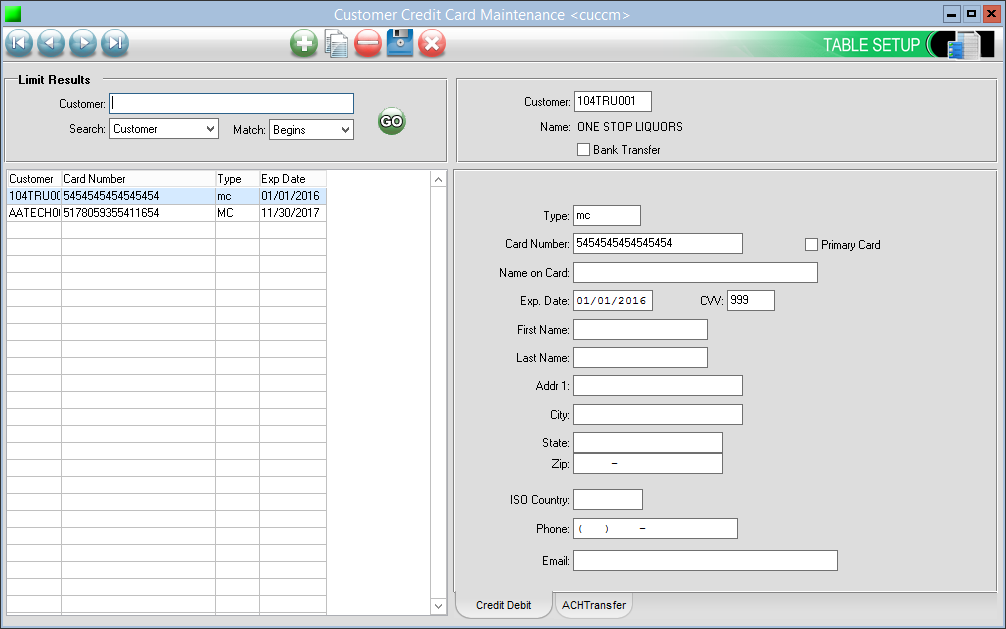
\includegraphics[width=\textwidth]{../img/image91}
	\caption{CUCCM Customer Credit Card Maintenance}
\end{figure}

If a customer pays by credit card for their orders and wants to store their credit card information with you, you may enter it here.

\subsection{Sales Order}

\subsubsection{Sales Order Entry}

\index{ERP-One Commands!OE}

The \texttt{OE} command is used to access Order Entry.

Information on the Order Entry screen will default in, set by the data and required fields you entered in customer setup (\texttt{CUMM}.) You are able to override these fields in order entry.

\begin{enumerate}
	\item Top Buttons
	\begin{itemize}
		\item Accept \textemdash Complete order by clicking \textbf{Accept}, order number will change to permanent order number
		\item Delete \textemdash Delete entire order
		\item Bill Order \textemdash Click \textbf{Bill Order} to process payment
		\item Convert Quote \textemdash Click \textbf{Convert Quote} to convert this order to a quote, you will be prompted with steps to convert to a quote
	\end{itemize}
	
	\begin{figure}[H]
		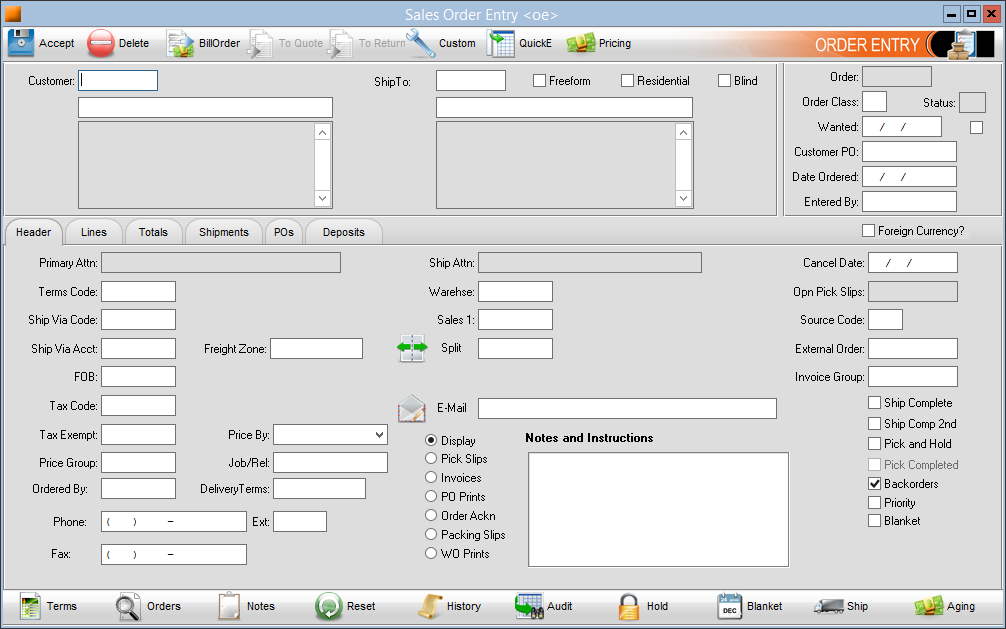
\includegraphics[width=\textwidth]{../img/image92}
		\caption{OE Sales Order Entry Header Tab}
	\end{figure}
	
	\item Header Tab
	\begin{itemize}
		\item Customer \textemdash Customer code, use F1 to search
		\item Ship To \textemdash Use F1 to select Ship To
		\item Address Options
		\begin{itemize}
			\item Freeform \textemdash To add a ship to in order entry, check freeform, add address, then hover over and click on ship to to add as a permanent record
			\item Residential \textemdash Choose residential indicator for shipper
			\item Blind \textemdash Ship blind, packing slip will show customer's ship to address
		\end{itemize}
		\item Order \textemdash Temporary order number will be automatically generated
		\item Order Class \textemdash Required field, default autofilled. Use F1 to open \texttt{OEOCM}
		\item Status \textemdash Status of order:
		\begin{itemize}
			\item CH \textemdash Credit Hold
			\item CL \textemdash Closed
			\item HO \textemdash Order Hold
			\item IV \textemdash Invoice
			\item OE \textemdash Order Entry
		\end{itemize}
		\item Wanted \textemdash Date the customer expects order delivered
		\item Customer PO \textemdash If PO is required, you must enter customer PO number
		\item Date Ordered \textemdash Current date auto-populates, use F1 to open calendar
		\item Entered By \textemdash Defaults to current user
		\item Terms Code \textemdash Required field, use F1 to open \texttt{SYTCM}
		\item Ship Via Code \textemdash Use F1 to open \texttt{SYSVM}
		\item Ship Via Acct \textemdash Enter customer shipping account if required
		\item Tax Code \textemdash Required field, use F1 to open \texttt{CUTXM}
		\item Ordered By \textemdash Customer contact, or use F1 to open list of alternate contacts for customer. Add new contact by hovering over Ordered By and click button that appears
		\item Warehse \textemdash Required field, autofills or use F1 to open \texttt{WAM}
		\item Sales 1 \textemdash Required field, use F1 to open \texttt{CUSRM}
		\item Source Code \textemdash Used to determine how the order was obtained.
		\item External Order \textemdash Web order number
		\item Check Boxes
		\begin{itemize}
			\item Ship Complete \textemdash Items will be allocated from stock, but order will not print until it can be filled 100\%
			\item Ship Comp $2^{nd}$ \textemdash Items in stock will print on first pick slip, backordered items will be allocated as they come into stock and second pick slip will be printed when order is 100\% filled.
			\item Pick and Hold \textemdash Items will be allocated, and pick ticket will be printed so that items can be placed into a staging area until the order is 100\% filled.
			\item Backorders \textemdash If checked, items will be backordered and printed on new pick slip as they come into stock.
		\end{itemize}
		\item Terms \textemdash Summary of terms / discounts with customer for this order
		\item Notes \textemdash Notes can be entered at time of order entry, per order or line item
		\item Aging \textemdash Summary of customer aging, indicates current or late payment		
	\end{itemize}
	
	\begin{figure}[H]
		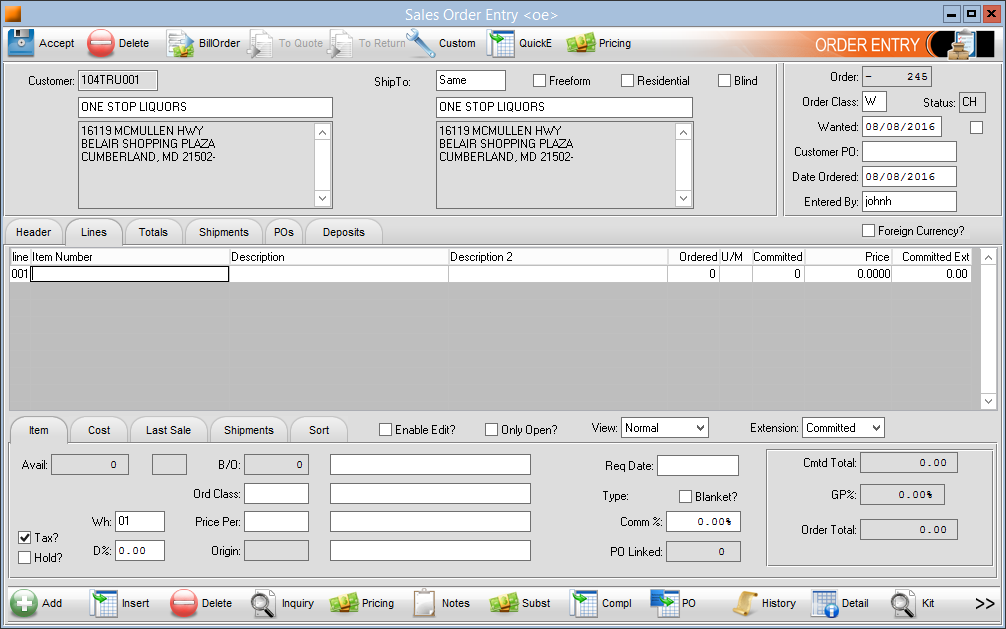
\includegraphics[width=\textwidth]{../img/image93}
		\caption{OE Sales Order Entry Lines Tab}
	\end{figure}
	
	\begin{figure}[H]
		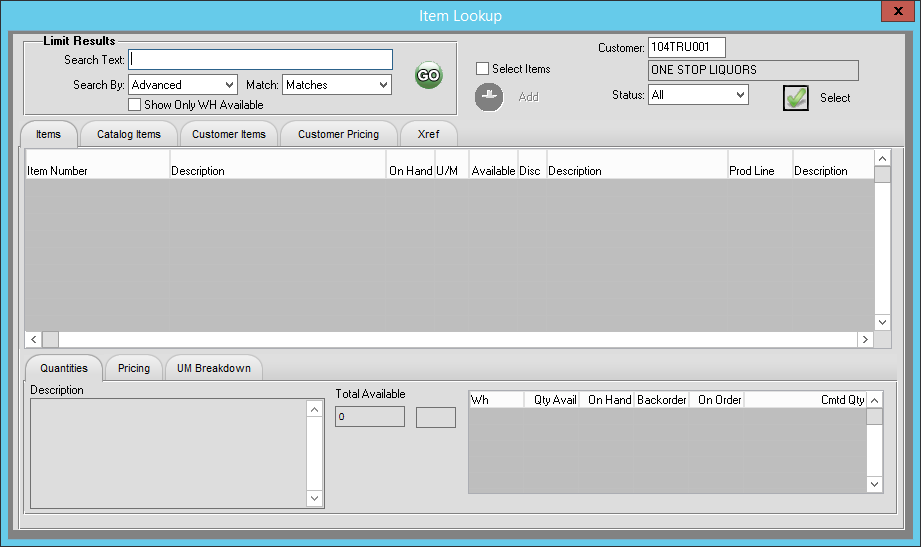
\includegraphics[width=\textwidth]{../img/image94}
		\caption{Product Lookup}
	\end{figure}	
	
	\item Lines Tab
	\begin{itemize}
		\item Line \textemdash Click on \textbf{add} to add line items
		\begin{itemize}		
			\item Item Number \textemdash Enter item number or use F1 to open item search
			\item Description \textemdash Description of item will appear here
		\end{itemize}
		\item Item Tab
		\begin{itemize}
			\item Tax? \textemdash If checked the item is taxable
			\item Wh \textemdash Which warehouse the item is located in
			\item D\% \textemdash Default discount for line item, you are able to add or override discount
			\item PRC \textemdash Order pricing options for gross profit
		\end{itemize}
		\item Cost Tab \textemdash Displays cost of item
		\item Last Sale Tab \textemdash Display price of item last time it was sold to this customer		
	\end{itemize}
	\item Bottom Buttons Under Lines Tab
	\begin{itemize}
		\item Add \textemdash Add line item
		\item Insert \textemdash Insert a new line item between two existing items
		\item Delete \textemdash Delete highlighted line item(s)
		\item Inquiry \textemdash Open \texttt{WAINQ} for highlighted line item
		\item Pricing \textemdash Display pricing information for highlighted line item
		\item Item Notes \textemdash Used to add notes at the line item level
		\item History \textemdash Display customer item purchase history for line item
		\item $\gg$
		\begin{itemize}
			\item Save Options \textemdash Save screen options you have changed for this login
			\item Assembly kit information for line item
			\item Lot and location information for line item
		\end{itemize}
	\end{itemize}
	
	\begin{figure}[H]
		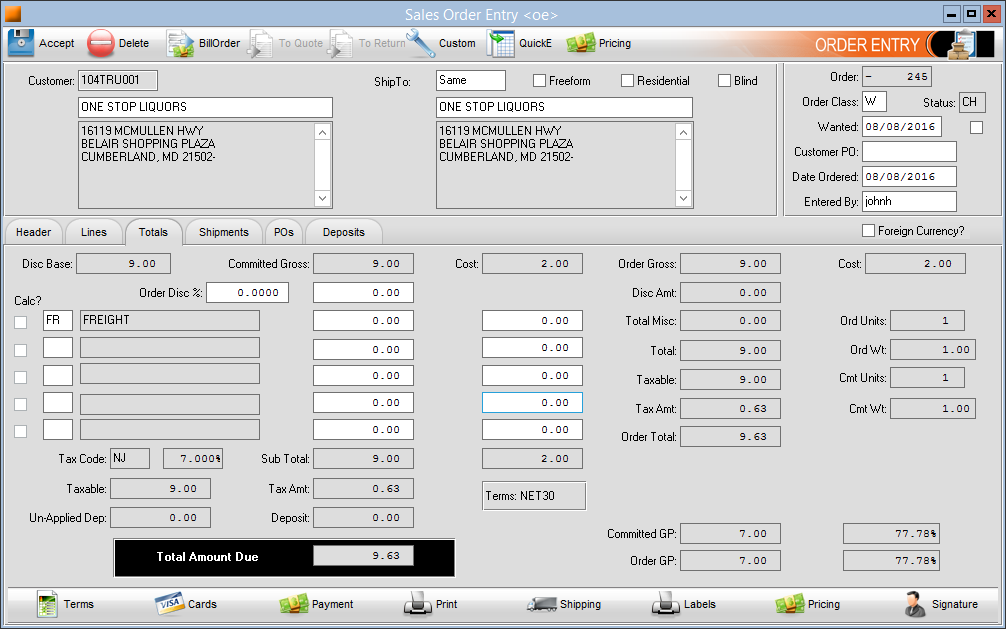
\includegraphics[width=\textwidth]{../img/image95}
		\caption{OE Sales Order Entry Totals Tab}
	\end{figure}	
	
	\item Totals Tab
	\begin{itemize}
		\item Additional Charges \textemdash Using F1 in this field will open \texttt{OETCM} to allow selection of any additional charge types
		\item Tax Code \textemdash Tax code defaults from header screen to this field
		\item Taxable \textemdash Calculated amount of tax
		\item Un-Applied Dep \textemdash Displays deposit paid to be applied to invoice
		\item Total Amount Due \textemdash Total amount due, including shipping, discounts and tax		
	\end{itemize}
	
	\begin{figure}[H]
		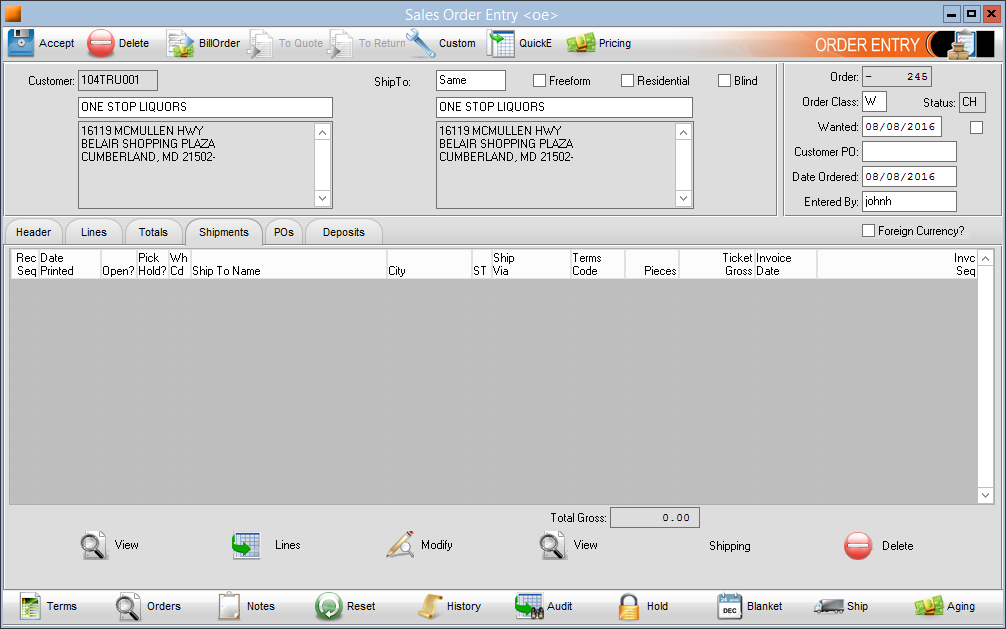
\includegraphics[width=\textwidth]{../img/image96}
		\caption{OE Sales Order Entry Shipments Tab}
	\end{figure}	
	
	\item Shipments Tab
	\begin{itemize}
		\item View Ship \textemdash Opens \texttt{OEIS}
		\item Lines \textemdash Displays lines in shipment
		\item Modify \textemdash Modify shipment
		\item View Inv \textemdash View invoice associated with shipment
		\item Shipping \textemdash Displays tracking and shipping information
		\item Delete \textemdash Deletes shipment record
	\end{itemize}
\end{enumerate}

\subsubsection{Order Lookup and Inquiry}

\index{ERP-One Commands!OEINQ}

The \texttt{OEINQ} command can is used to access Order Lookup and Inquiry

\begin{figure}[H]
	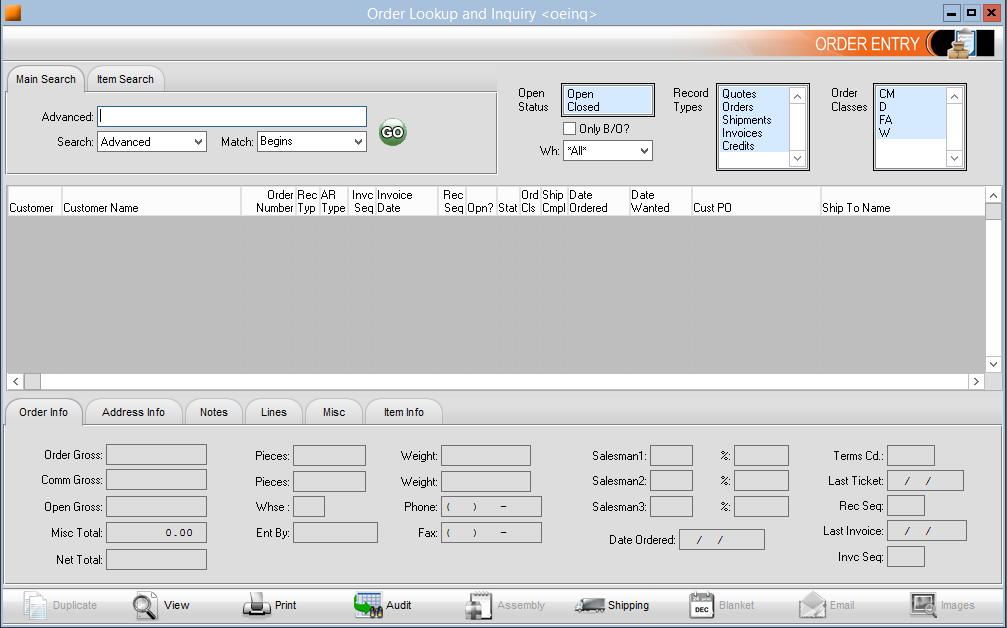
\includegraphics[width=\textwidth]{../img/image5}
	\caption{OEINQ Order Inquiry Screen}
\end{figure}

\begin{itemize}
	\item Open Status \textemdash Search within the status of the order
	\begin{itemize}
		\item Open
		\item Closed
		\item Only B/O? \textemdash If checked, search only orders with backorders
	\end{itemize}
	\item Record Type \textemdash Type of order you want to search through
	\begin{itemize}
		\item Quotes
		\item Orders
		\item Shipments
		\item Invoices
		\item Credits
	\end{itemize}	
	\item Order Class \textemdash Class of order to search, list is managed using \texttt{OEOCM}
	\begin{itemize}
		\item D \textemdash Direct Ship
		\item N \textemdash Rental
		\item W \textemdash From Warehouse
		\item C \textemdash Commission
	\end{itemize}
	\item Results View
	\begin{itemize}
		\item Customer Name
		\item Order Number
		\item Record Type \textemdash An identifier of what type of record is being displayed
		\begin{itemize}
			\item Q \textemdash Quotes
			\item O \textemdash Order
			\item I \textemdash Invoice
			\item S \textemdash Shipment
			\item C \textemdash Credit
		\end{itemize}
		\item Record Sequence \textemdash The number sequence of the document
		\item Invoice Date \textemdash Date Invoices
		\item Order Class
		\item Ship Complete \textemdash Indicates if order was specified to ship complete
		\item Date Ordered
		\item Date Wanted
		\item Cust PO
	\end{itemize}
	\item Bottom Buttons
	\begin{itemize}
		\item View \textemdash View the highlighted order. Opens \texttt{OE} screen for that order.
		\item Print \textemdash Reprint or re-send a document
		\item Audit \textemdash View complete audit for highlighted record
		\item Shipping \textemdash Displays shipment information for order
	\end{itemize}
\end{itemize}

\subsection{Purchase Order}

\subsubsection{Purchase Order Entry}

\index{ERP-One Commands!POE}

The commant \texttt{POE} is used to access Purchase Order Entry.

Information on your purchase order entry screen will auto populate or be filled in by the information entered furing vendor setup in \texttt{VEMM}. The defaulted fields in purchase order entry can be overridden.

\begin{enumerate}
	\item Entry Fields \textemdash Your purchase order will automatically generate a temporary number in the system that will be used until you accept the order.
	\begin{itemize}
		\item Order Class \textemdash Required field. Using F1 opens \texttt{POOCM}
		\item Status \textemdash Status of the order
		\item Date Wanted \textemdash Date you are expecting the order to arrive
		\item Cancel Date \textemdash Date to cancel PO if it has not been received
		\item Date Ordered \textemdash Current date is autofilled. Use F1 to open calendar to choose other date.
		\item Entered By \textemdash Populated with current user id
	\end{itemize}
	\item Top Buttons
	\begin{itemize}
		\item Accept \textemdash Accepts order, temporary purchase order number will be replaced with permanent number
		\item Delete \textemdash Deletes entire order
	\end{itemize}
	
	\begin{figure}[H]
		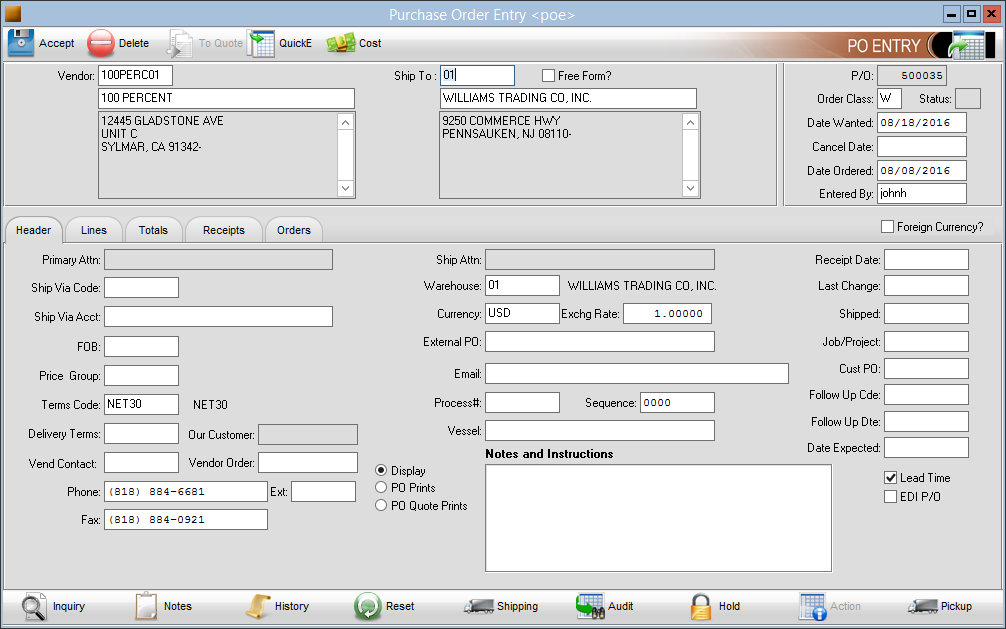
\includegraphics[width=\textwidth]{../img/image97}
		\caption{POE Purchase Order Entry Header Tab}
	\end{figure}
	
	\item Header Tab
	\begin{itemize}
		\item Vendor Field \textemdash Enter vendor code or use F1 to search for vendor.
		\item Ship Via Code \textemdash The shipping method to request for this order, use F1 to open \texttt{SYSVM}
		\item Ship Via Acct \textemdash Optional. The shipping account number to use for shipment.
		\item Terms Code \textemdash Required field. Using F1 opens \texttt{SYTCM}
		\item Warehouse \textemdash Where order is being sent. Using F1 opens \texttt{WAM}	
		\item Follow Up
		\begin{itemize}
			\item Follow Up Code \textemdash Using F1 opens \texttt{POFLOH}
			\item Follow Up Date \textemdash Date to follow up with vendor on status of order if not yet received
			\item Date Expected \textemdash Date of expected delivery of order
		\end{itemize}
		\item Bottom Buttons
		\begin{itemize}
			\item Notes \textemdash Notes can be entered at time of purchase order entry, per order or line item
		\end{itemize}
	\end{itemize}
	
	\begin{figure}[H]
		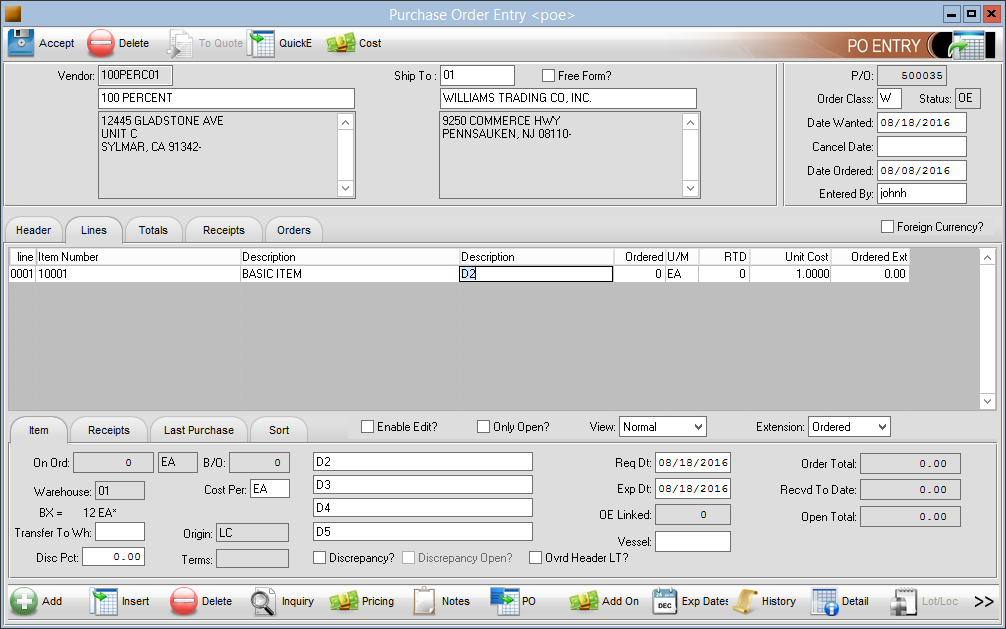
\includegraphics[width=\textwidth]{../img/image98}
		\caption{POE Purchase Order Entry Lines Tab}
	\end{figure}
	
	\item Lines Tab \textemdash Click on the add icon at the bottom to add line items
	\begin{itemize}
		\item Item Number \textemdash Enter item number or use F1 to open item search
		\item Description \textemdash Description of item will appear here
		\item Enable Edit? \textemdash If checked, the cost and other item fields may be modified
	\end{itemize}
	\item Bottom Tabs
	\begin{itemize}
		\item Item
		\begin{itemize}
			\item On Ord \textemdash Quantity of items on all open PO's
			\item Wh \textemdash Warehouse item is located
			\item Disc Pct \textemdash Default discount for line item, able to add or override
			\item B/O \textemdash Quantity on backorder
		\end{itemize}
		\item Cost Per \textemdash Cost per U/M of item
	\end{itemize}
	\item Bottom Buttons
	\begin{itemize}
		\item Add \textemdash Add line item
		\item Insert \textemdash Insert a line item between existing lines
		\item Delete \textemdash Delete selected line item(s)
		\item Inquiry \textemdash Open \texttt{WAINQ} for selected item
		\item Pricing \textemdash Pricing for selected item
		\item Notes \textemdash Add note to selected line item
		\item Exp Date \textemdash Displays expected dates and quantities for line item
		\item $\gg$
		\begin{itemize}
			\item Save Options \textemdash Save screen options you have created
		\end{itemize}
	\end{itemize}
	
	\begin{figure}[H]
		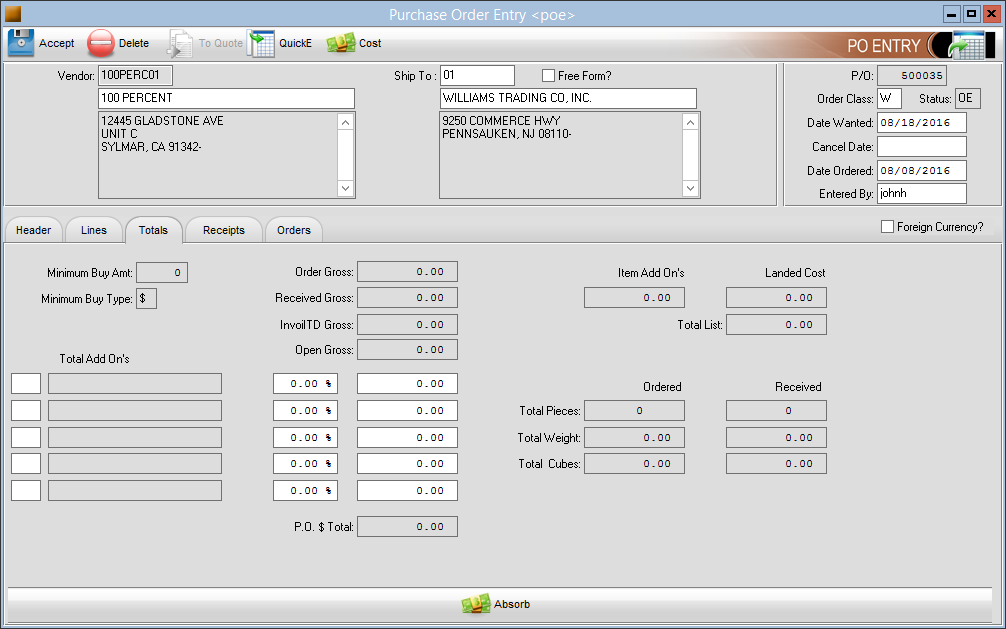
\includegraphics[width=\textwidth]{../img/image99}
		\caption{POE Purchase Order Entry Totals Tab}
	\end{figure}
	
	\item Totals Tab
	\begin{itemize}
		\item Total Add On's / Additional Charges \textemdash Use F1 in this field to open \texttt{POACM} and select any additional charge type
		\item P.O. \$ Total \textemdash Total amount due, including shipping, discounts and tax
	\end{itemize}
\end{enumerate}

\subsubsection{Purchase Order Lookup and Inquiry}

\index{ERP-One Commands!POINQ}

The \texttt{POINQ} command is used to access Purchase Order Lookup and Inquiry.

\begin{figure}[H]
	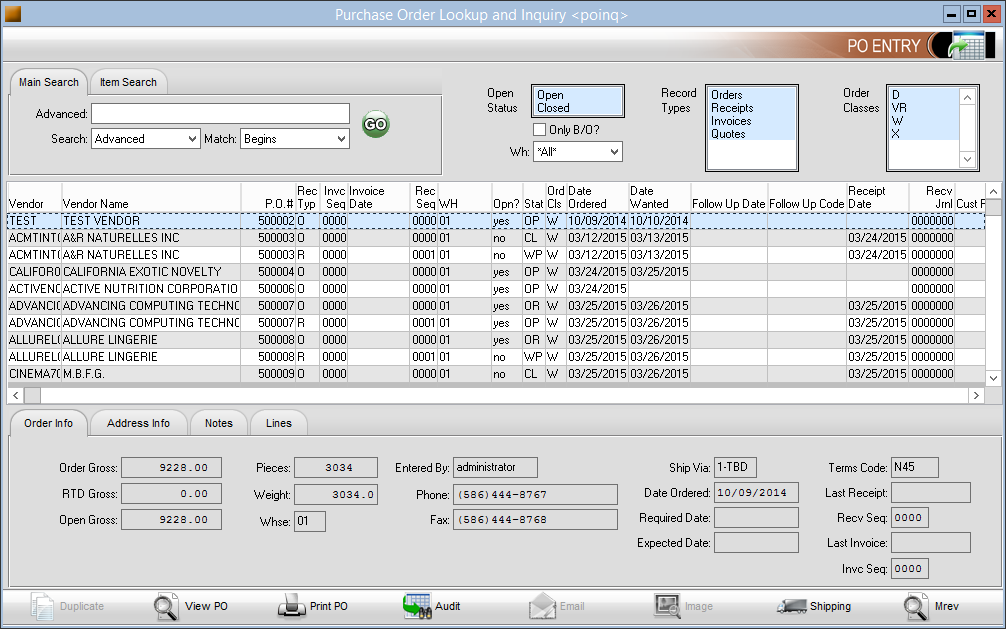
\includegraphics[width=\textwidth]{../img/image100}
	\caption{POINQ Purchase Order Lookup and Inquiry}
\end{figure}

\begin{itemize}
	\item Open Status \textemdash Search within the status of the order
	\begin{itemize}
		\item Open
		\item Closed
	\end{itemize}
	\item Record Type \textemdash Type of order you want to search through
	\begin{itemize}
		\item Quotes
		\item Orders
		\item Invoices
		\item Receipts
	\end{itemize}	
	\item Order Class \textemdash Class of order to search, list is managed using \texttt{OEOCM}
	\begin{itemize}
		\item D \textemdash Direct Ship
		\item W \textemdash From Warehouse
		\item X \textemdash Vendor Returns
	\end{itemize}
	\item Only B/O? \textemdash If checked, search only orders with backorders
	\item Results View
	\begin{itemize}
		\item Vendor Name
		\item Purchase Order Number
		\item Record Type \textemdash An identifier of what type of record is being displayed
		\begin{itemize}
			\item Q \textemdash Quotes
			\item O \textemdash Order
			\item I \textemdash Invoice
			\item R \textemdash Receipts
		\end{itemize}
		\item Record Sequence \textemdash The number sequence of the document
		\item Invoice Date \textemdash Date Invoices
		\item Order Class
		\item Date Ordered
		\item Date Wanted
	\end{itemize}
	\item Bottom Buttons
	\begin{itemize}
		\item View PO \textemdash View the highlighted order. Opens \texttt{POII} screen for that order.
		\item Print \textemdash Reprint or re-send a document
		\item Audit \textemdash View complete audit for highlighted record
	\end{itemize}
\end{itemize}

\subsubsection{Purchase Order Suggested Buy}

\index{ERP-One Commands!POSB}

\begin{figure}[H]
	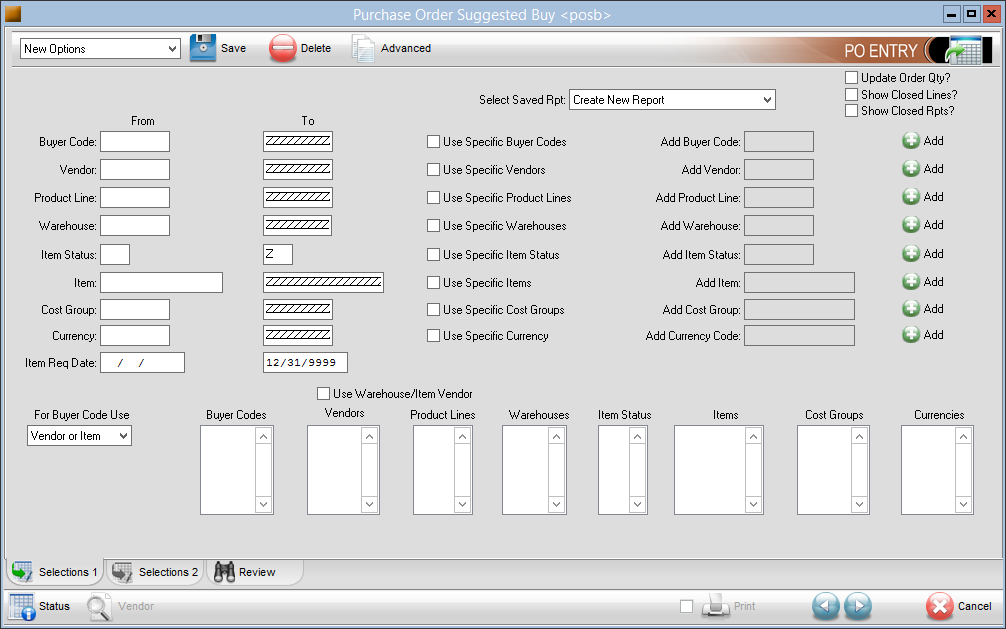
\includegraphics[width=\textwidth]{../img/image101}
	\caption{POSB Purchase Order Suggested Buy}
\end{figure}

\begin{enumerate}
	\item Selections 1 \textemdash This screen allows for the selection of criteria for items that will appear in the review
	\item Selections 2 \textemdash Further options for review
	\item Review \textemdash This will process and show the resulting list of items that need to be purchased
	\begin{itemize}
		\item Vendor List \textemdash This is the default vendor for the item
		\item Item List \textemdash These are the items needed from the highlighted vendor
	\end{itemize}
\end{enumerate}

\subsection{Information Inquiry Reference}

\subsubsection{Inventory Inquiry}

\index{ERP-One Commands!WAINQ}

Looking up information about items in the warehouse may be accomplished using the \texttt{WAINQ} command.

\begin{figure}[H]
	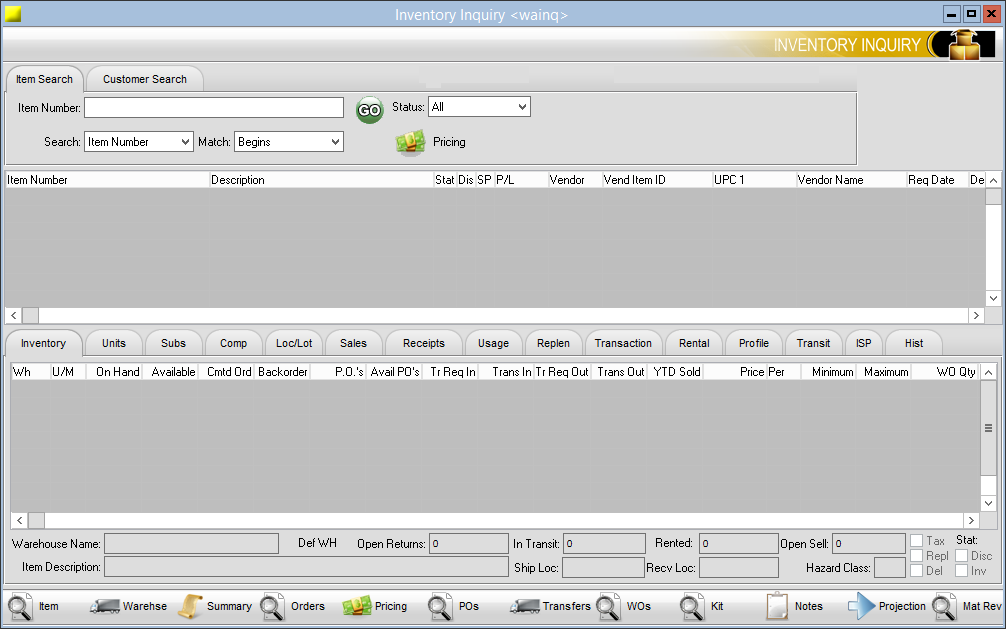
\includegraphics[width=\textwidth]{../img/image53}
	\caption{WAINQ Inventory Inquiry}
\end{figure}

The default search settings will allow you to search for items by their item number. Changing the \textbf{Search} and \textbf{Match} dropdown options will allow you to perform advanced searches for items.

\begin{figure}[H]
	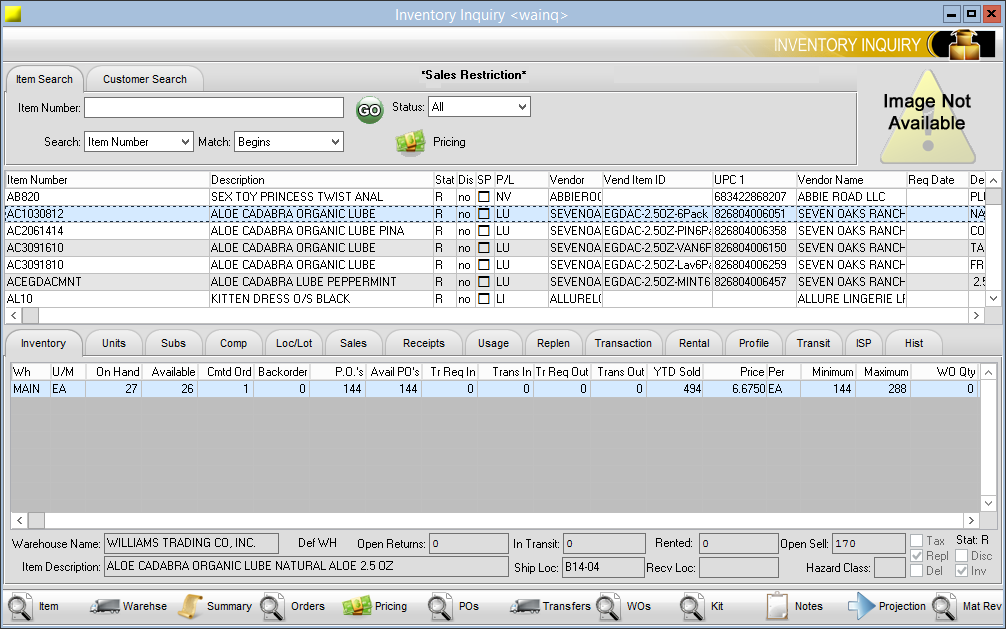
\includegraphics[width=\textwidth]{../img/image54}
	\caption{WAINQ Inventory Inquiry Detail}
\end{figure}

Selecting an item will display detail about that item.

\subsubsection{Order Lookup}

\index{ERP-One Commands!OEINQ}

Looking up information regarding an order that has been entered into the system is straight-forward. The \texttt{OEINQ} command in ERP-ONE will allow you to view the progress of any order and access any documents.

\begin{figure}[H]
	\includegraphics[width=\textwidth]{../img/image5}
	\caption{OEINQ Order Inquiry Screen}
\end{figure}

You may search for an order by the order number, the website order number, the customer's purchase order number, and many more.  Be sure to select 'Advanced' and 'Matches' in the Search and Match drop down boxes if you are having difficulty finding an order without access to the order number.

When you find an order, you may click on it to view the following information:

\begin{figure}[H]
	\includegraphics[width=\textwidth]{../img/image6}
	\caption{OEINQ Order Inquiry Screen with order selected}
\end{figure}

The \textbf{Audit} and \textbf{Shipping} buttons will allow you to view useful information to the customer when providing status updates on their order.

You can also easily access detailed customer information by right clicking on the order, and selecting \textbf{Drill to...} which will give you the option to view the \textbf{Customer Inquiry} and \textbf{Sales History Inquiry} for that customer.

\begin{figure}[H]
	\includegraphics[width=\textwidth]{../img/image7}
	\caption{OEINQ Drill To options}
\end{figure}

\index{ERP-One Commands!CUI}

Selecting \textbf{Customer Inquiry} will direct you to the Customer Inquiry screen that allows you to view the current payment status of the customer.

\begin{figure}[H]
	\includegraphics[width=\textwidth]{../img/image8}
	\caption{CUI Customer Inquiry}
\end{figure}


\section{Warehouse Manager Console}

The Warehouse Manager Console is located at http://wms/ you may only access this console from within the local area network.

\subsection{Dashboard}

The dashboard includes four charts of information, showing the overall fulfilment rate of both E-Commerce and Wholesale orders and the current top selling products.

\subsection{Document Tracker}

The Document Tracker is used to move order / pick-list printouts from the office to the warehouse. Users can use the terminal by the interior warehouse door to scan paperwork in and out of the bins.

\subsection{Picker Log}

The Picker Log is used to track pick-list assignment.  Warehouse employees are required to scan their pick-lists and record the number of pages and lines that they received.  There also is a Picker Log (Single) interface for recording single wholesale orders being picked, the page and line counts will be recorded automatically.

\subsection{Product Lookup}

Employees may use the Product Lookup feature to find complete information about products in the warehouse, including images and descriptions.

\subsection{Order Lookup}

All known order information can be looked up in the Order Lookup section, which will show carton contents, and individual tracking information for each carton, along with dimensions and freight charges.  There is also a Order Lookup (MFG) for MFG orders.

\subsection{Committed Products}

Committed Products shows a list of all items currently on pick-lists in the warehouse, you can search and sort this list.

\subsection{Open Shipment Report}

The Open Shipment Report shows all current open shipments in the warehouse.
